\chapter{Irradiation test for superconducting magnet material}
~~~~~Since the superconducting solenoid of COMET experiment is exposed under the high radiation environment, the superconducting solenoid has a risk of quench due to the radiation damage in the some part of solenoid.
Thus, the study of radiation damage on the material used in COMET superconducting magnet system is quite significant.
In this chapter, the irradiation test on GFRPs, Quench protection diode and pure aluminium will be introduced.

 \section{Glass Fiber Reinforced Plastic}
~~~~~Glass Fiber Reinforced Plastics (GFRP) are widely used in many engineering applications because of their superior properties such as higher specific strength, specific modulus, anti-corrosion and thermal insulation~\cite{gfrp}.
In the case of COMET experiment, GFRPs are employed as the insulation spacer for superconducting magnets which suffer high magnetic field and radiation.
Due to the worse radiation resistance for the Glass-Epoxy (G10), 3 kinds of GFRPs what impregnate the Bismaleimide-Triazine (BT), Bismaleimide (BMI) and Cyanate Ester (CE) in the S-2 glass fiber have been developed to enhance the radiation resistance and mechanical properties.
Here Boron is excluded from the S-2 glass in order to reduce the influence from neutron.

 \subsection{Experiment}
~~~~~Each sample of GFRPs (G10, CE, BT and BMI) is prepared as Japanese Industrial Standards (JIS), which is with 100 mm long, 10 mm wide and 0.5 mm thick.
The irradiation test of GFRPs is taken in the Takasaki Advanced Radiation Research Institute by using 1 MeV uniform electron beam and Research Reactor Institute, Kyoto University (KUR) by using 34 MeV accelerator electron beam.
After irradiation, the tensile strength of irradiated samples is measured as well.
Figure~\ref{3samplegfrp} shows how GFRP samples break after irradiation.

For the 1 MeV electron irradiation test, radiation dose is measured by cellulose triacetate (CTA) tape~\cite{cta} and it can be estimated from the equation as follows.
\begin{equation}
 dose = \frac{D_e - D_0}{K} \cdot \frac{0.125}{t} \cdot f
\end{equation}
where the unit of dose is kGy.
$D_e$ and $D_0$ is the light absorption before and after irradiation.
$K$ is the constant for irradiation which is defined to 0.0063 for electron and 0.0081 for photon.
$t$ and $f$ are the thickness of CTA tape and correction term, respectively.
Average radiation dose is about 0.8 kGy/sec$\cdot$mA in terms of this equation.
Each sample of G10, CE, BT and BMI is irradiation with 50, 100 and 200 MGy totally.
As the results shown in figure~\ref{3resultgfrp} (left), BT and BMI are definitely stronger than G10 and CE without irradiation.
The tensile strength of G10 and CE drops to about 150 MPa after 200 MGy irradiation.
Similarly, BMI also has a tendency to degrade.
While the BT, the tensile strength has no big change after 200 MGy irradiation.
 \begin{figure}[H]
  \begin{subfigure}{0.22\textwidth}
   \centering
   \includegraphics[scale=0.28]{chapter4/fig/gfrp.eps}
  \end{subfigure}
  \hspace{0.2\textwidth}
  \begin{subfigure}{0.22\textwidth}
   \centering
   \includegraphics[scale=0.33]{chapter4/fig/broke.eps}
  \end{subfigure}
  \caption{GFRP samples before the irradiation are shown on the left. The samples are tensioned until break after irradiation (right).}
  \label{3samplegfrp}
 \end{figure}
\begin{figure}[H]
  \begin{subfigure}{0.3\textwidth}
   \centering
   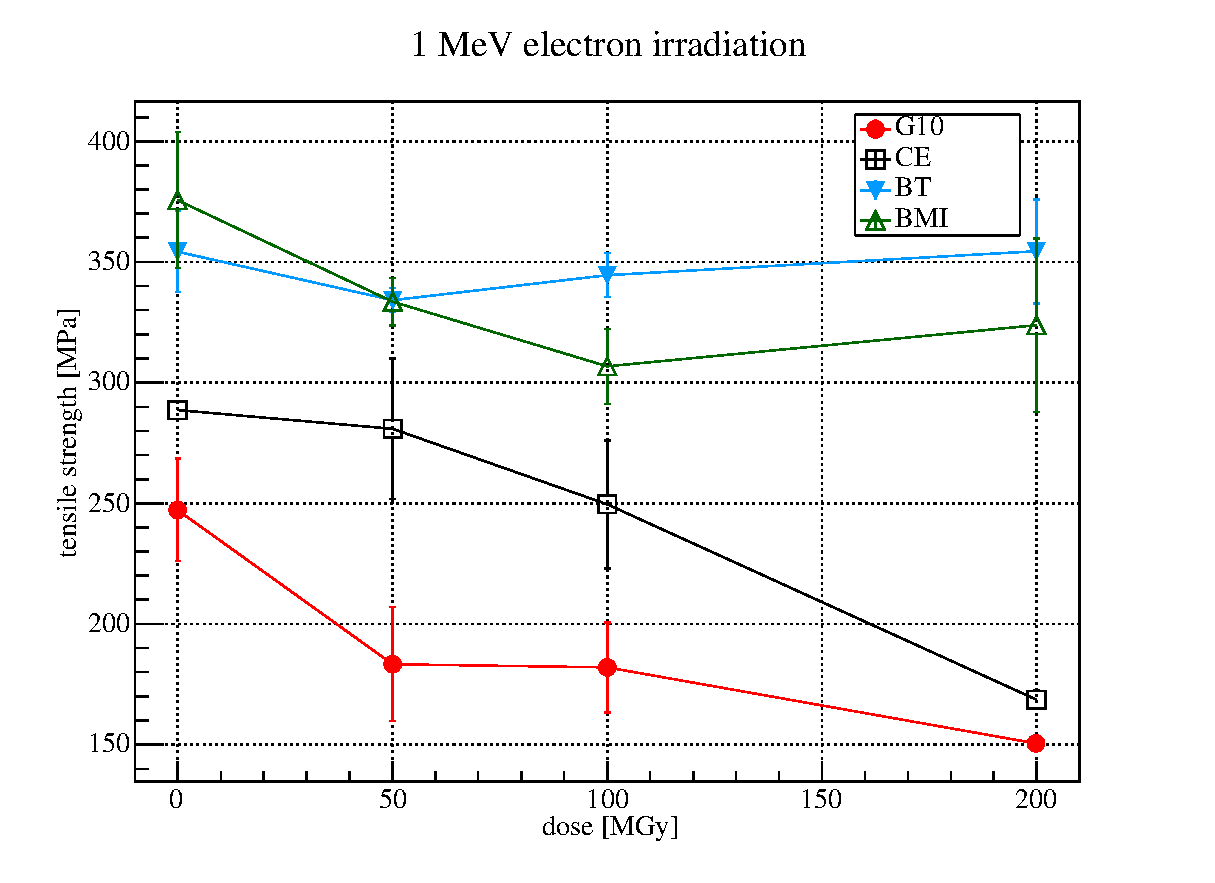
\includegraphics[scale=0.43]{chapter4/fig/tensile_takasaki.eps}
  \end{subfigure}
  \hspace{0.2\textwidth}
  \begin{subfigure}{0.3\textwidth}
   \centering
   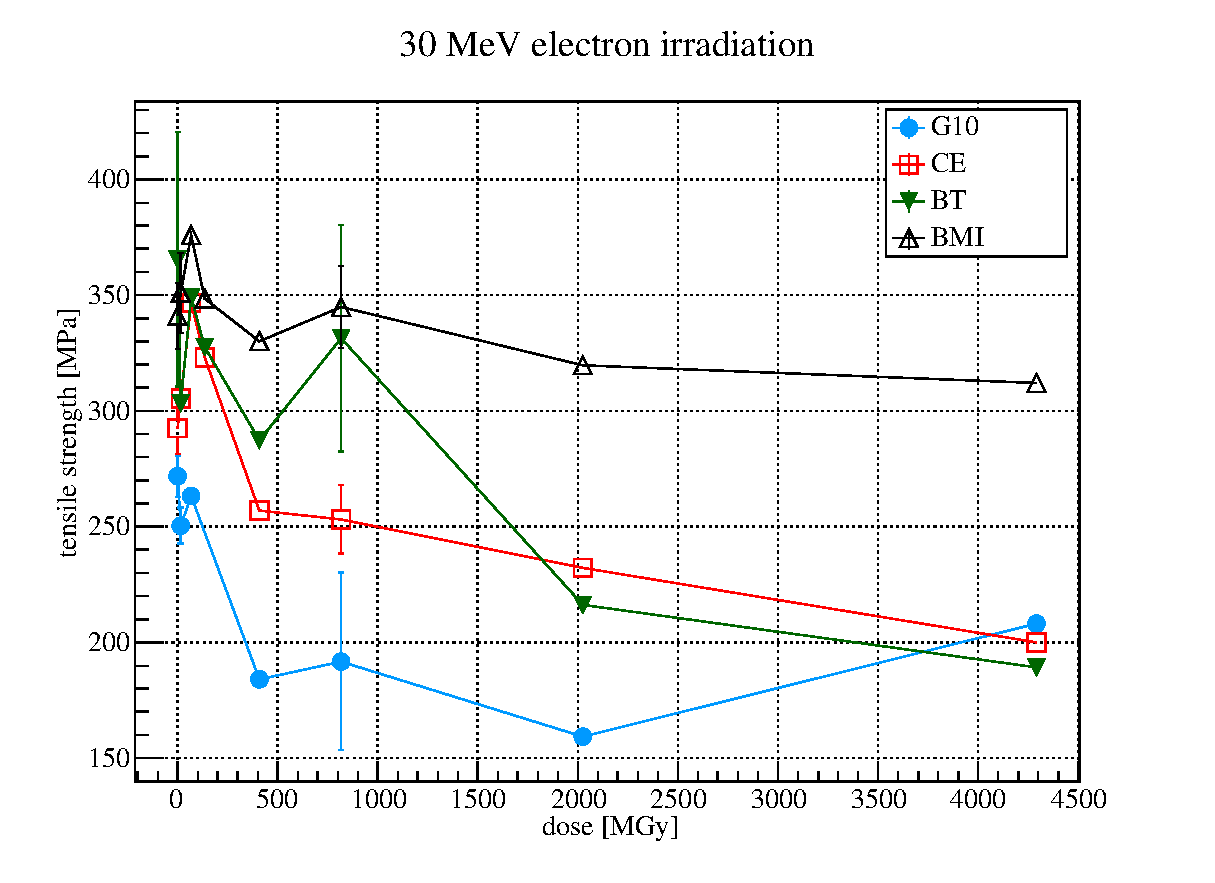
\includegraphics[scale=0.43]{chapter4/fig/tensile_kyoto.eps}
  \end{subfigure}
  \caption{The tensile strength of irradiated samples (G10, CE, BMI and BT) when it breaks. Left and Right figure represent 1 MeV electron irradiation test in JAEA, Takasaki and 30 MeV electron irradiation test in LINAC, KURRI.}
  \label{3resultgfrp}
 \end{figure}
To investigate the reaction of high energy electron on GFRPs, irradiation with 34 MeV electron has been tested by using accelerator.
Because of the electron with high energy, not only the electron but also the photon from Bremsstrahlung and neutron from the photonuclear reaction interact on GFRPs.
LINAC accelerator at KUR provides a gaussian beam with the width of 30 mm.
GFRP sample is cooled by water during the irradiation (30$^{\circ}$C).
Unlike to the 1 MeV irradiation, CTA tape is unable to be used to measure the radiation dose because its energy is out of the range of the measurement ability of CTA tape.
Thus, in this case, radiation dose is estimated by PHITS code, which is 1.25 kGy/sec$\cdot$mA.
Each sample is irradiated with 9, 30, 45, 90, 270, 540, 1340 and 2840 MGy totally.
In figure~\ref{3resultgfrp}, all samples start to degrade from 90 MGy and they drop to around 200 MPa besides BMI.
The flexural strength test and outgasing test for GFRPs are described in reference~\cite{takasaki}.
Considering the mechanical property, outgasing and radiation resistance, BT will be employed as insulation spacer in COMET superconducting magnets.

\section{Insulation tape}
%~~~~~The conduct is commonly covered with several polyimide tapes as ground insulation between two conducts.
%As for the COMET superconducting magnets, 4 kinds of insulation tape, BTGU, BTGK-A, BTGK-B, BTGK-C, are developed to enhance the mechanical property and radiation resistance.
~~~~~~The conductor of pion capture solenoid is wound by two layers of insulation tape so called pre-preg tape as ground insulation.
This insulation tape shown in figure~\ref{3stur} is made of polyimide film covered by boron free glass with BT and epoxy resin to enhance the mechanical property under the high radiation environment.
 \begin{figure}[H]
  \begin{subfigure}{0.3\textwidth}
  \centering
  \includegraphics[scale=0.33]{chapter4/fig/preg.pdf}
  %\caption{ The structure of pre-preg tape.}
  \end{subfigure}
  \hspace{0.2\textwidth}
  \begin{subfigure}{0.3\textwidth}
  \centering
  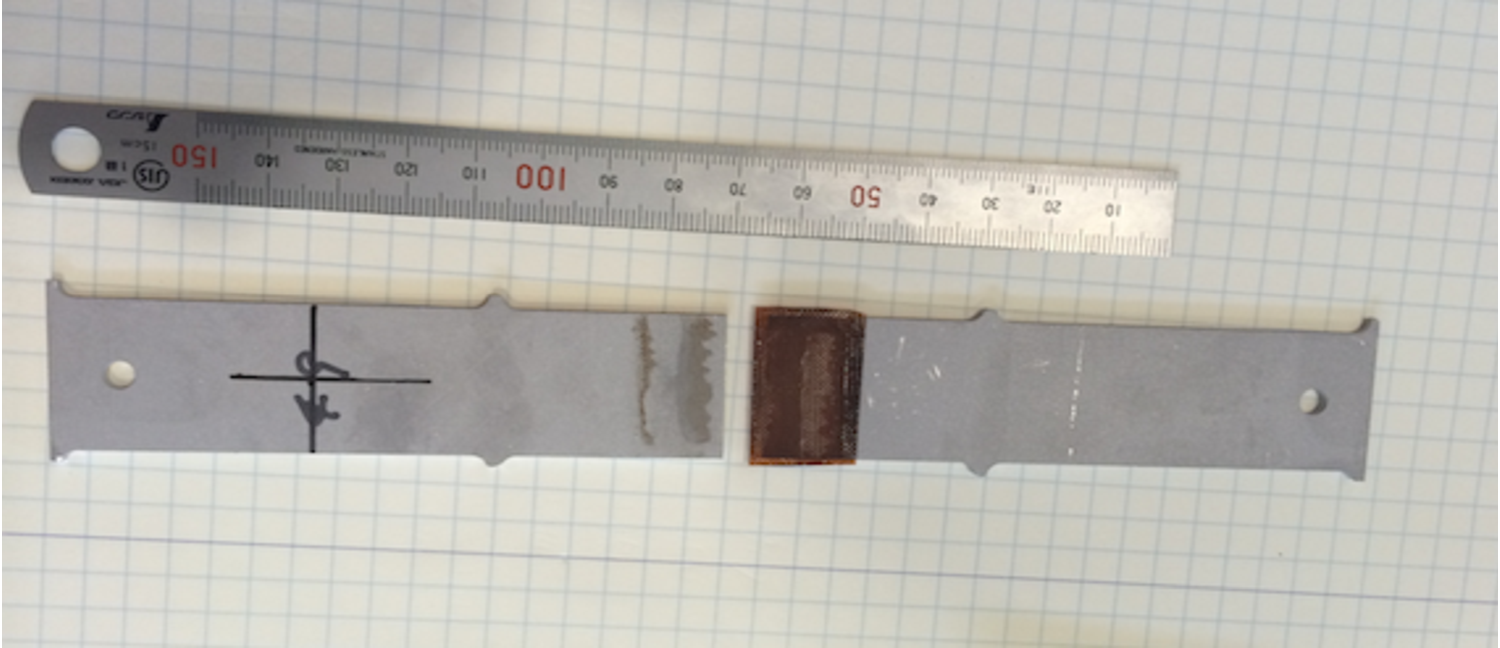
\includegraphics[scale=0.30]{chapter4/fig/BUGT.pdf}
  %\caption{ Tensile test for pre-preg tape.}
  \end{subfigure}
  \caption{Insulation tape is made of glass cross and polyimide film impregnated by BT and epoxy resin (left). The two pieces of insulation tapes are sandwiched with aluminium strip to take tensile test (right).}
 \label{3stur}
 \end{figure}
 \begin{figure}[H]
  \begin{subfigure}{0.3\textwidth}
   \centering
   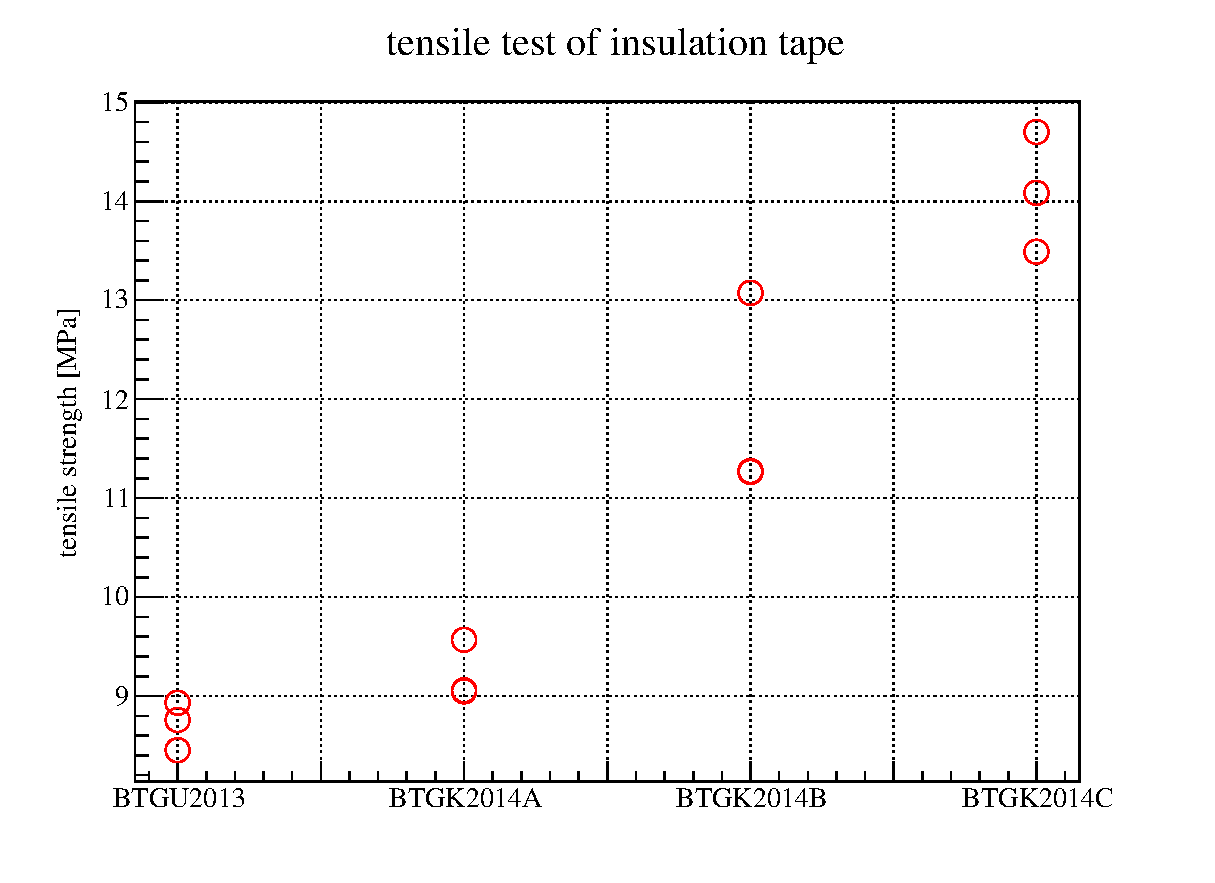
\includegraphics[scale=0.43]{chapter4/fig/gubt.eps}
  \end{subfigure}
  \hspace{0.2\textwidth}
  \begin{subfigure}{0.3\textwidth}
   \centering
   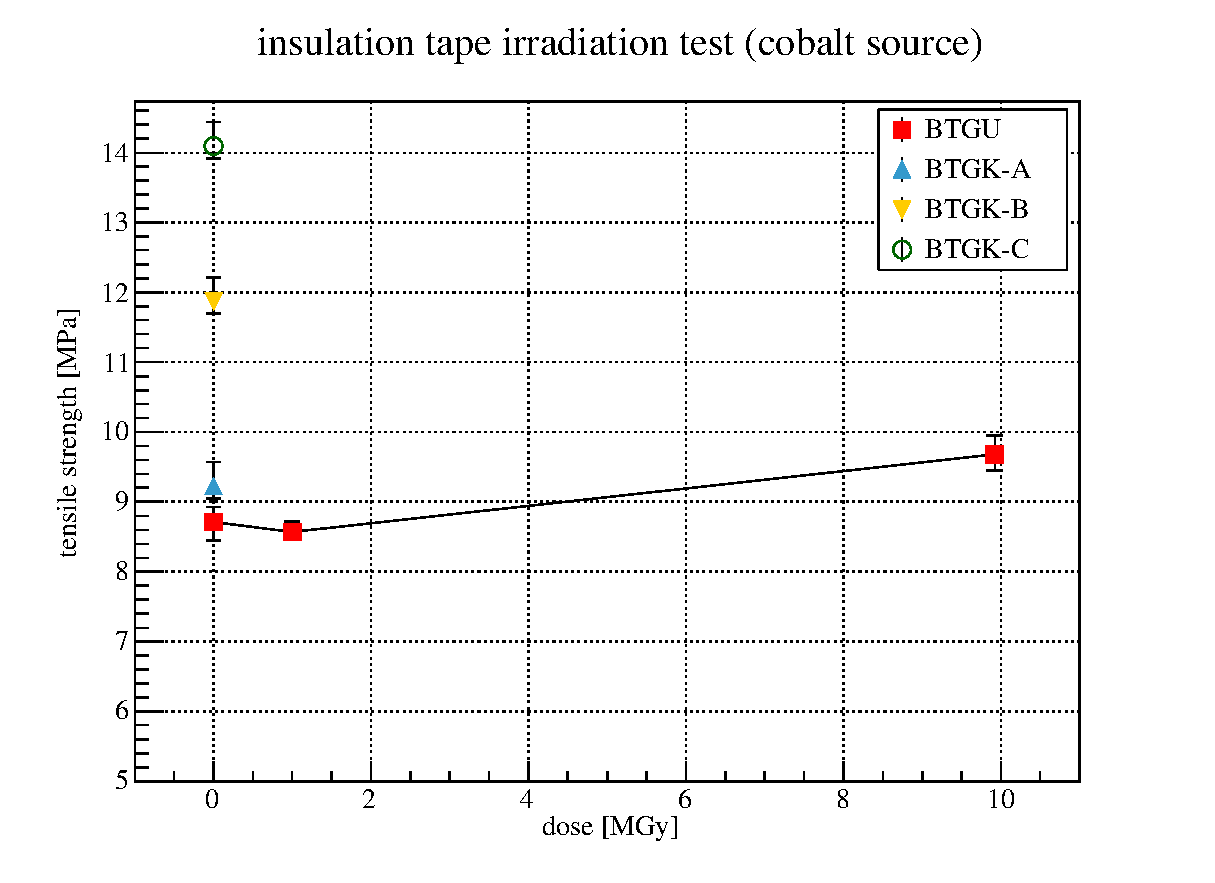
\includegraphics[scale=0.43]{chapter4/fig/BTGU2.eps}
  \end{subfigure}
  \caption{3 samples of each BTGU, BTGK-A, BTGK-B and BTGK-C are tensioned without irradiation (left). BTGU shows no degradation after irradiated with 10 MGy at limit by cobalt $\gamma$ ray source.}
  \label{3gubt}
 \end{figure}
Four samples, BTGU, BTGK-A, BTGK-B and BTGK-C, made of same material but different rate of BT and epoxy resin are prepared for tensile test.
Here, mixing the BT and epoxy resin with different rate can adjust the viscosity of insulation tape.
Two samples are struck and sandwiched with aluminium strip (Al-GU-UG-Al) as JIS standards for tensile test are cured by 170$^{\circ}$C and 8 hours.
Figure~\ref{3stur} shows how the pre-preg tape breaks after tensile test.

The result of tensile test for the sample without irradiation is given in figure~\ref{3gubt}, which shows the BTGK-C is the strongest one in these sample.
However, the glass layer and resin layer is not struck before the thermal process, which is hard to employ it as the insulation tape in superconducting coil.
Considering the mechanical properties may reduce after irradiation, the irradiation of BTGU samples is taken in Takasaki Advanced Radiation Research Institute with cobalt radiation source.
As the result shown in figure~\ref{3gubt} (right), the tensile strength of BTGU sample does not reduce after irradiation, however, surprisingly, the tensile strength increases about 10\% after 10 MGy irradiation.



% \section{Stabilizer and conductor}
%The early radiation induced damage on superconductors with reactor neutron is studied at cryogenic temperature by Weber~\cite{weber}.
%The results show that the critical current density of NbTi drops from 10$^{22}$ n/m$^2$ high energy neutron irradiation at 5 Tesla.
 \section{Quench protection diode}
~~~~~Quench protection diode is a switch of the dump resistor.
When magnets quench, the power supply will be cut off, then this diode will be turned on and current will flow toward the dump resistor.
The operating voltage will increase after irradiation~\cite{hagedorn}, which causes the over heat of quench protection diode.
Moreover different manufacturer fabricates diode with different electrical property.
Here, a dedicated quench protection diode for COMET superconducting magnet has been irradiated by high energy neutron.
Its electrical characteristics under low temperature and radiation is investigated.

  \subsection{Experiment}
~~~~~The irradiation test for quench protection diode is taken with COMET detector group together at the Tendem accelerator, Kyushu university.
The fast neutron is produced from carbon target with incident 9 MeV deutron, which creates neutron by deutron-deutron reaction.
5 kinds of samples are set up in front of the production target with the distance of 3 cm as the sequence of MPPC, APD, Artix-7, ROESTI and diode, which is shown in figure~\ref{3setup}.
 \begin{figure}[H]
  \centering
  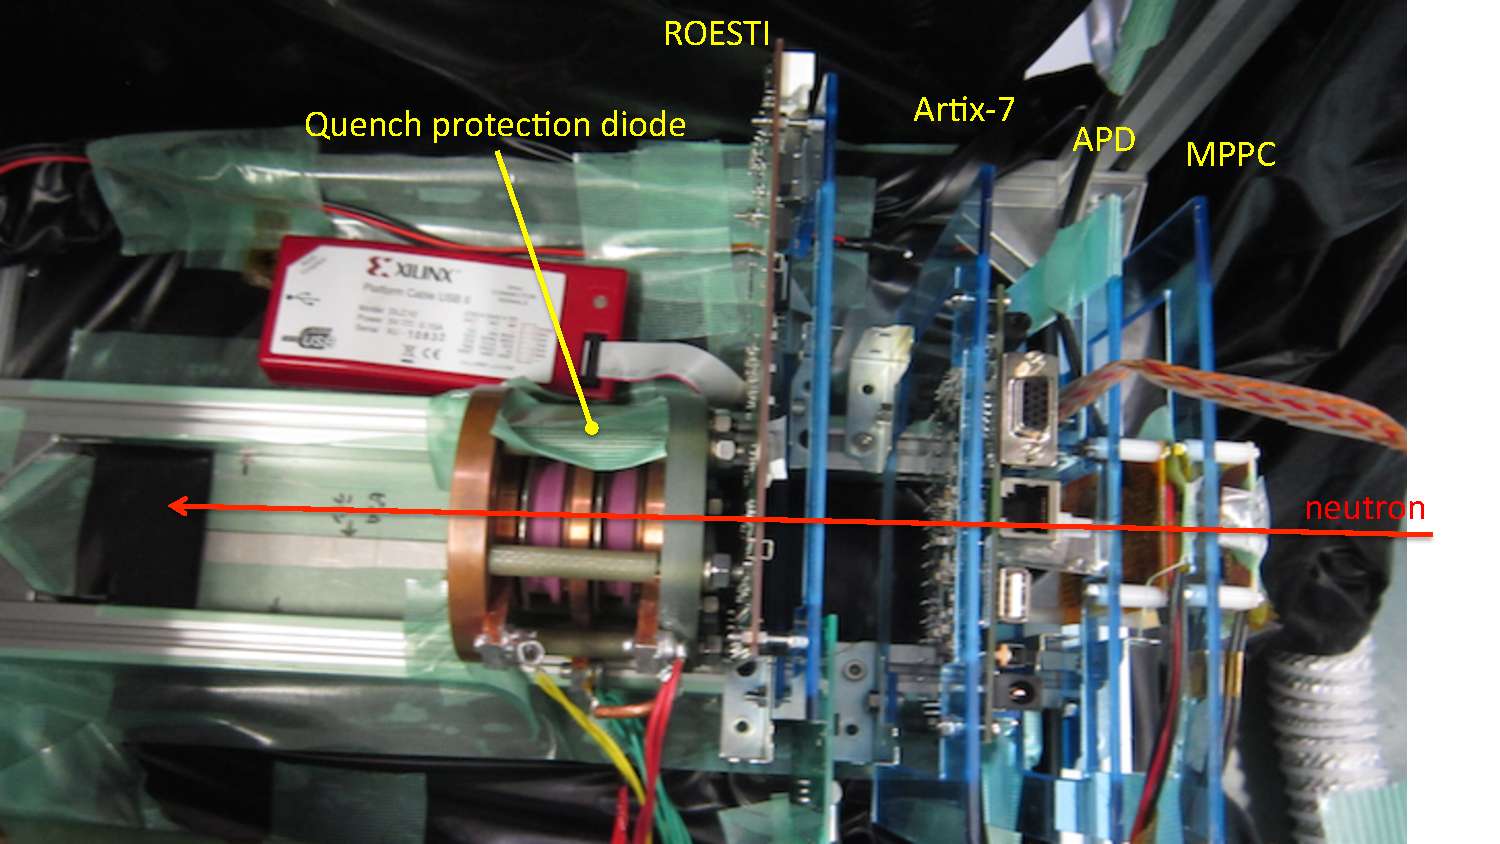
\includegraphics[scale=0.45]{chapter4/fig/diodepic.pdf}
  \caption{Sample setup for neutron irradiation test. Diode is set up in front of MPPC, APD, Artix-7 and ROESTI where is 30 cm far from the neutron production target.}
  \label{3setup}
 \end{figure}
Because diode is with the radius of 3 cm and length of 10 cm, which is possible to stop the neutron, it is located at last of samples where 30 cm far from the production target.
Its turn-on voltage is measured during the irradiation with 5 A power supply, and neutron flux is measured by activation analysis with aluminium, nickel and gold wire (0.07\% Fe).
Temperature of diode during the irradiation is recorded by thermometer.
  
  \subsection{Neutron measurement}
~~~~~Activation analysis is a common and easy way of neutron measurement, but with the bad energy resolution.
aluminium, nickel and gold wire (0.07\% Fe) are employed and stuck on the surface of each sample.
The photon from neutron reaction on each activation sample which is list in table~\ref{act} is measured by HPGe detector.
\begin{table}[H]
 \centering
 \begin{tabular}{ccccc} \hline \hline
  Element & Reaction & Threshold energy & Half life & Emitted radiation energy [MeV] \\ \hline
  aluminium & $^{27}$Al(n, p)$^{27}$Mg & 1.9 MeV & 9.46 min & $\beta^-$ (1.75), $\gamma$ (0.84, 1.013) \\
  aluminium & $^{27}$Al(n, $\alpha$)$^{24}$Na & 3.27 MeV & 15 h & $\beta^-$ (1.389), $\gamma$ (1.369, 2.754) \\
  Gold & $^{197}$Au(n, $\gamma$)$^{198}$Au & (-) & 2.7 d & $\beta^-$ (0.962), $\gamma$ (0.412) \\
  Gold & $^{197}$Au(n, 2n)$^{196}$Au & 7.36 MeV & 6.18 d & $\beta^-$, $\gamma$ (0.356) \\
  Nickel & $^{58}$Ni(n, 2n)$^{57}$Ni & 12.09 MeV & 36 h & $\beta^+$, $\gamma$ (0.511, 1.37) \\ \hline \hline
 \end{tabular}
 \caption{Neutron activation reactions.}
 \label{act}
\end{table}
  \begin{figure}[H]
   \begin{subfigure}{0.3\textwidth}
    \centering
	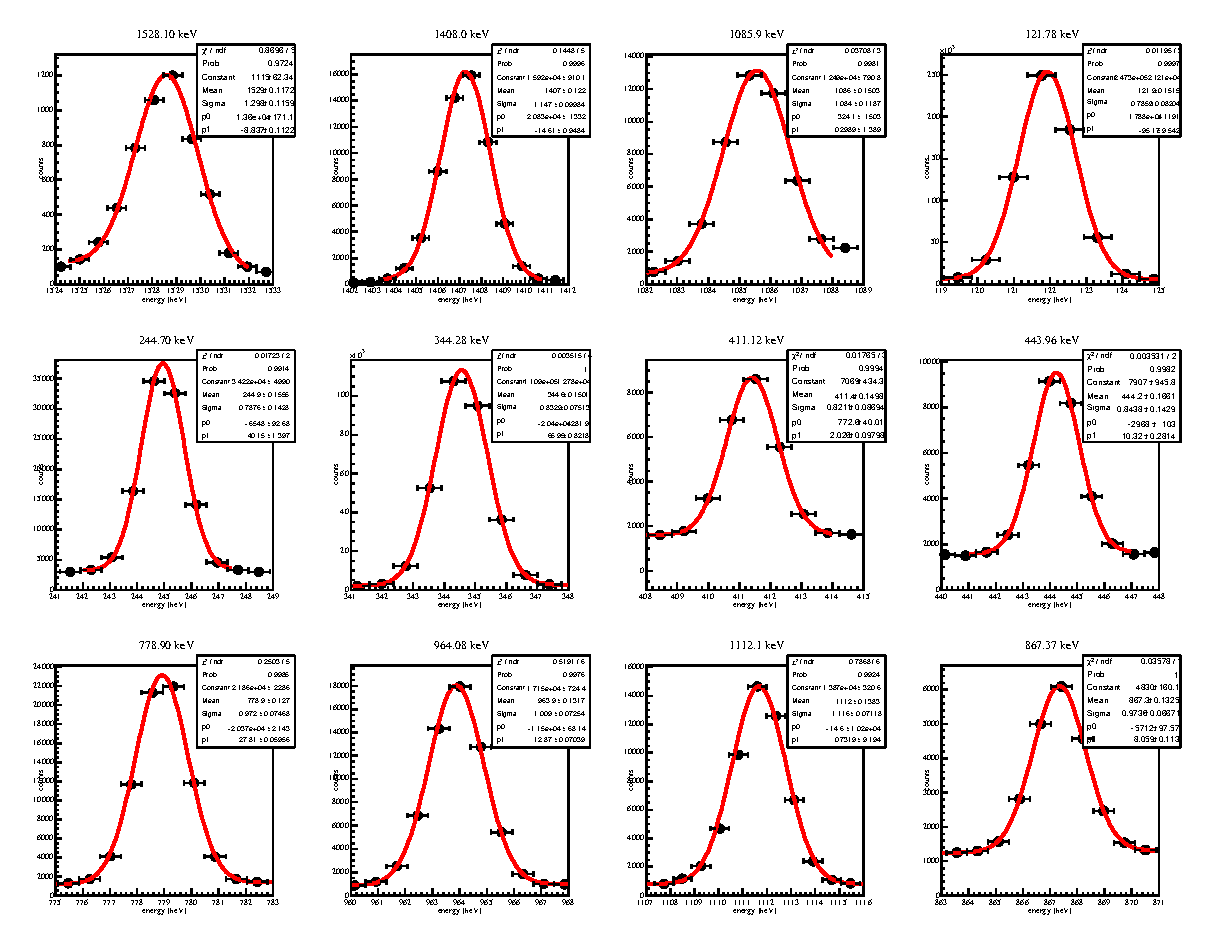
\includegraphics[scale=0.46]{chapter4/fig/Eufit.eps}
   \end{subfigure}
   \hspace{0.25\textwidth}
   \begin{subfigure}{0.3\textwidth}
    \centering
	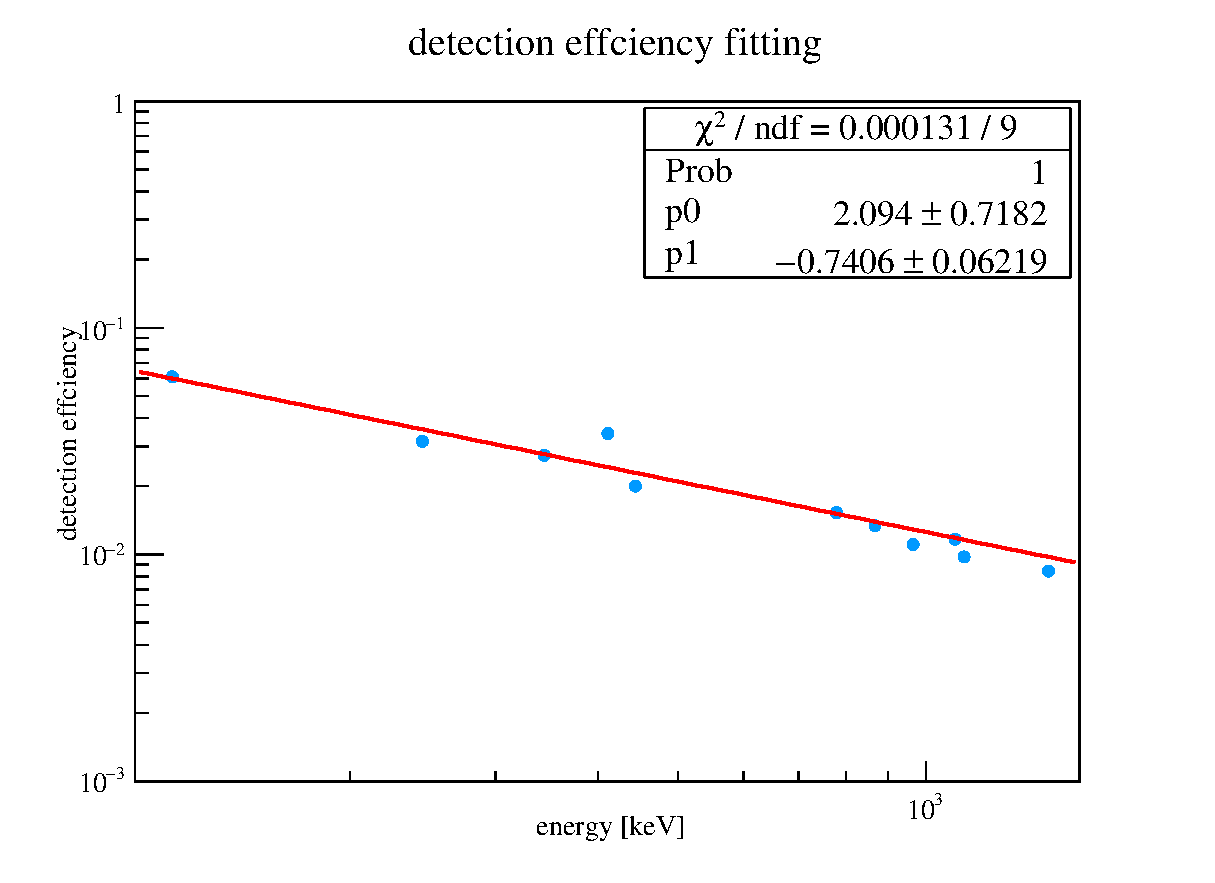
\includegraphics[scale=0.35]{chapter4/fig/detectioneff.eps}
   \end{subfigure}
   \caption{The detection efficiency is calibrated by using $^{152}$Eu radiation source. Several peak of $^{152}$Eu is fitted as convolution on left, and the detection efficiency of HPGe is fitted on right.}
   \label{3source}
  \end{figure}
$^{152}$Eu with 2.79$\times$10$^7$ Bq is employed as the calibration source to estimate the detection efficiency of HPGe detector.
As shown in figure~\ref{3source}, each peak of radiation source $^{152}$Eu is fitted as gaussian and linear function.
The detection efficiency is fitted as
\begin{equation}
 \epsilon = a \cdot E^b
\end{equation}
where the counts for the calculation of detection efficiency $\epsilon$ is within 1.78$\sigma$.
\begin{table}[H]
 \centering
 \begin{tabular}{cc} \hline \hline
  a & b \\ \hline
  2.094$\pm$0.7182 & -0.7406$\pm$0.06219 \\ \hline \hline
 \end{tabular}
 \caption{Fitting parameters for detection efficiency.}
\end{table}

%  \begin{figure}[H]
%   \centering
%   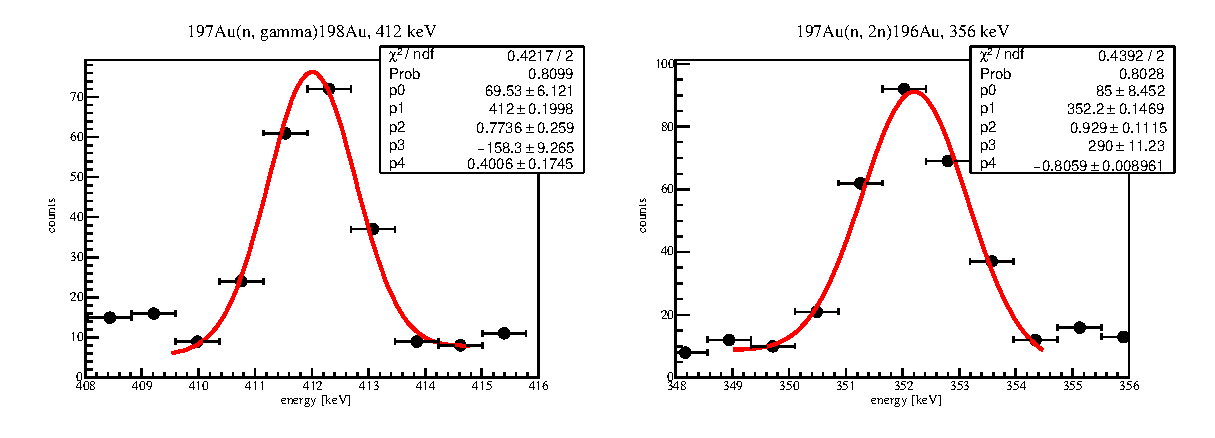
\includegraphics[scale=0.45]{chapter4/fig/aupeak}
%   \caption{ The peak of $^{197}$Au decay on the diode downstream.}
%   \label{3nipeak}
%  \end{figure}

Neutron flux measured by each activation sample is given by~\cite{nicholas}
\begin{equation}
 \phi = \frac{C \cdot A \cdot \lambda}{\sigma \cdot N_A \cdot \gamma \cdot m \cdot I \cdot \epsilon \cdot (1 - e^{-\lambda t_0}) \cdot (e^{-\lambda t_1} - e^{-\lambda t_2})}
\end{equation}
where $C$ is the number of counts under the peak of each activation sample.
$\sigma$ and $\gamma$ are the cross section of a reaction which is picked up from JENDL data library and probability that a photon is emitted per decay of the isotope respectively.
$N_A$ is the Avogadro constant, and $I$ is a weight fraction of isotope with atomic mass $A$.
$m$ is the mass of activation sample.
$\epsilon$ and $t_2-t_1$ are the detection efficiency and counting time.
  \begin{figure}[H]
   \begin{subfigure}{0.3\textwidth}
   \centering
   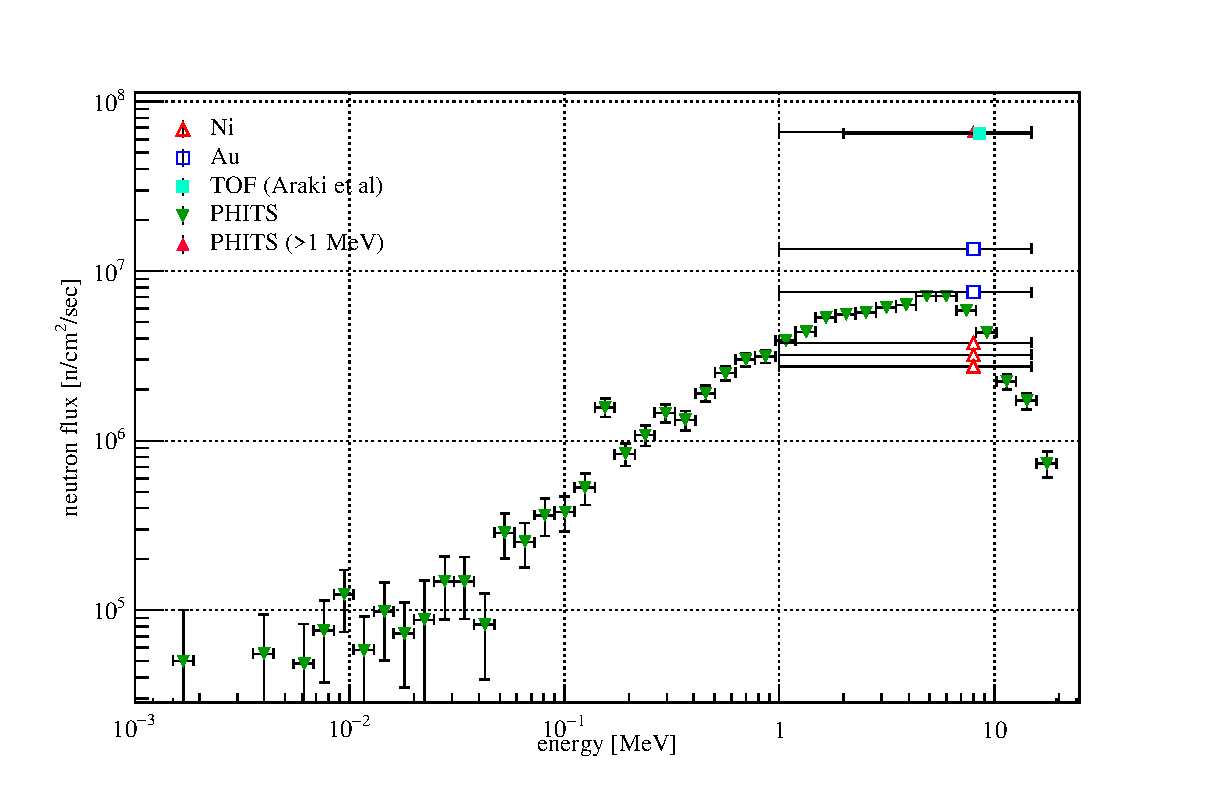
\includegraphics[scale=0.45]{chapter4/fig/flux}
   \end{subfigure}
   \hspace{0.2\textwidth}
   \begin{subfigure}{0.3\textwidth}
   \centering
   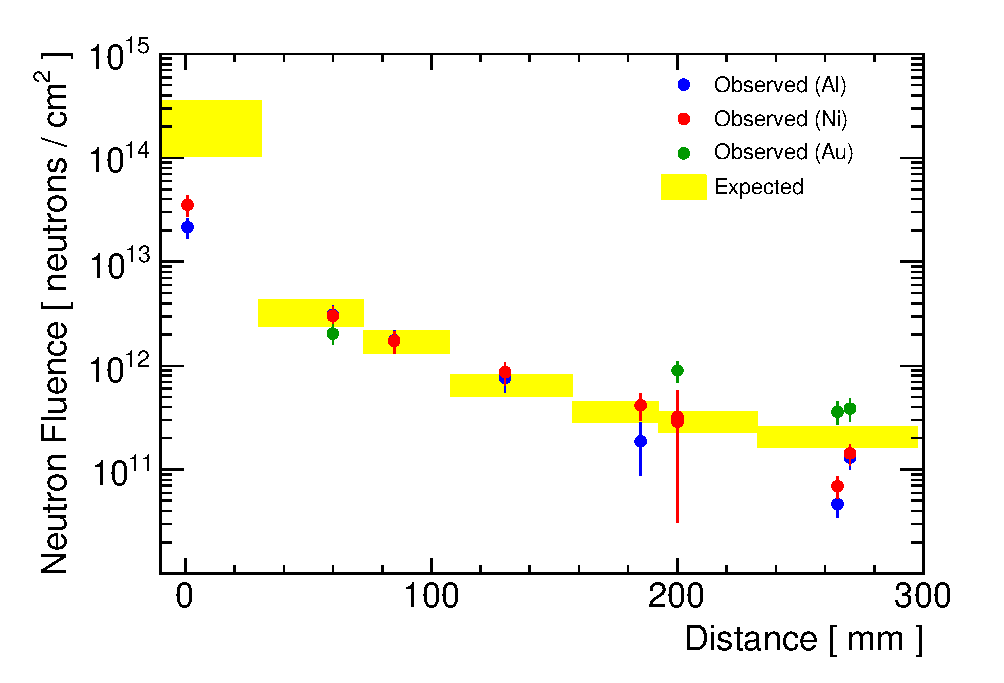
\includegraphics[scale=0.48]{chapter4/fig/fluxtot.pdf}
   \end{subfigure}
   \caption{Neutron flux is measured by Au wire, Al and Ni foils. The comparison of experimental data with simulation (left). The neutron flux on the place where samples are set up is shown on rihgt.}
   \label{3flux}
  \end{figure}

As shown in figure~\ref{3flux}, neutron flux on diode measured by gold wire is higher nickel's, which is 1.35$\times$10$^7$ n/cm$^2$/sec.
From the prediction of PHITS code and previous measurement with liquid scintillator, the neutron flux is 6$\times$10$^7$ n/cm$^2$/sec which is about 5 times higher than the measurement of gold wire.
It is possible that a part of neutron is stopped at flange or the other irradiation sample and causes the different between measurement and prediction.
Thus, in this case, we trust the measurement and the total neutron fluence irradiated until the end of experiment is estimated for 10$^{12}$ n/cm$^2$.

  \subsection{Electrical property of diode}
~~~~~To investigate the electrical properties of diode, the turn-on voltage is measured during the irradiation, then the voltage on the operating current is predicted by fitting the V-I curve of diode.
The relation of turn-on voltage (forward voltage at 100 mA) and neutron fluence is shown in figure~\ref{3switch}.
It reduces with neutron fluence and slope of V-I curve becomes bigger after irradiation.
Temperature from the beginning of the experiment until the end of the experiment is controlled around 25.6$^{\circ}$C.

Figure~\ref{3fitdiode} shows the fitting for each V-I curve as the function~\ref{dioeq}, and fitting parameters are listed in table~\ref{fit3}.
\begin{equation}
 I = I_0 (e^{-V/V_T} - 1)
\label{dioeq}
\end{equation}
where $I$ and $V$ are the diode current and voltage across the diode.
$V_T$ is thermal voltage and $I_0$ is the saturation current, which are assumed the fitting parameters here.
  \begin{figure}[H]
   \begin{subfigure}{0.3\textwidth}
    \centering
	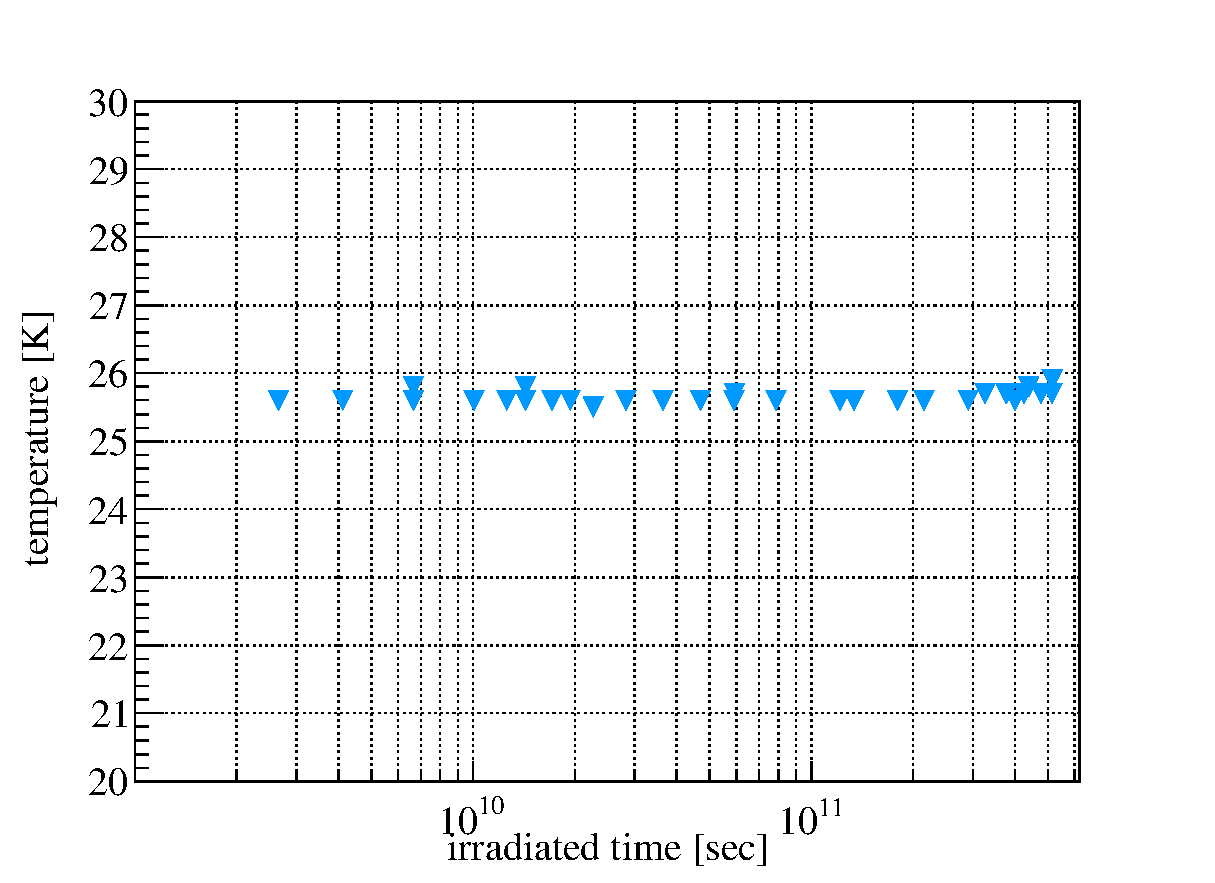
\includegraphics[scale=0.43]{chapter4/fig/temperature.eps}
   \end{subfigure}
   \hspace{0.2\textwidth}
   \begin{subfigure}{0.3\textwidth}
    \centering
	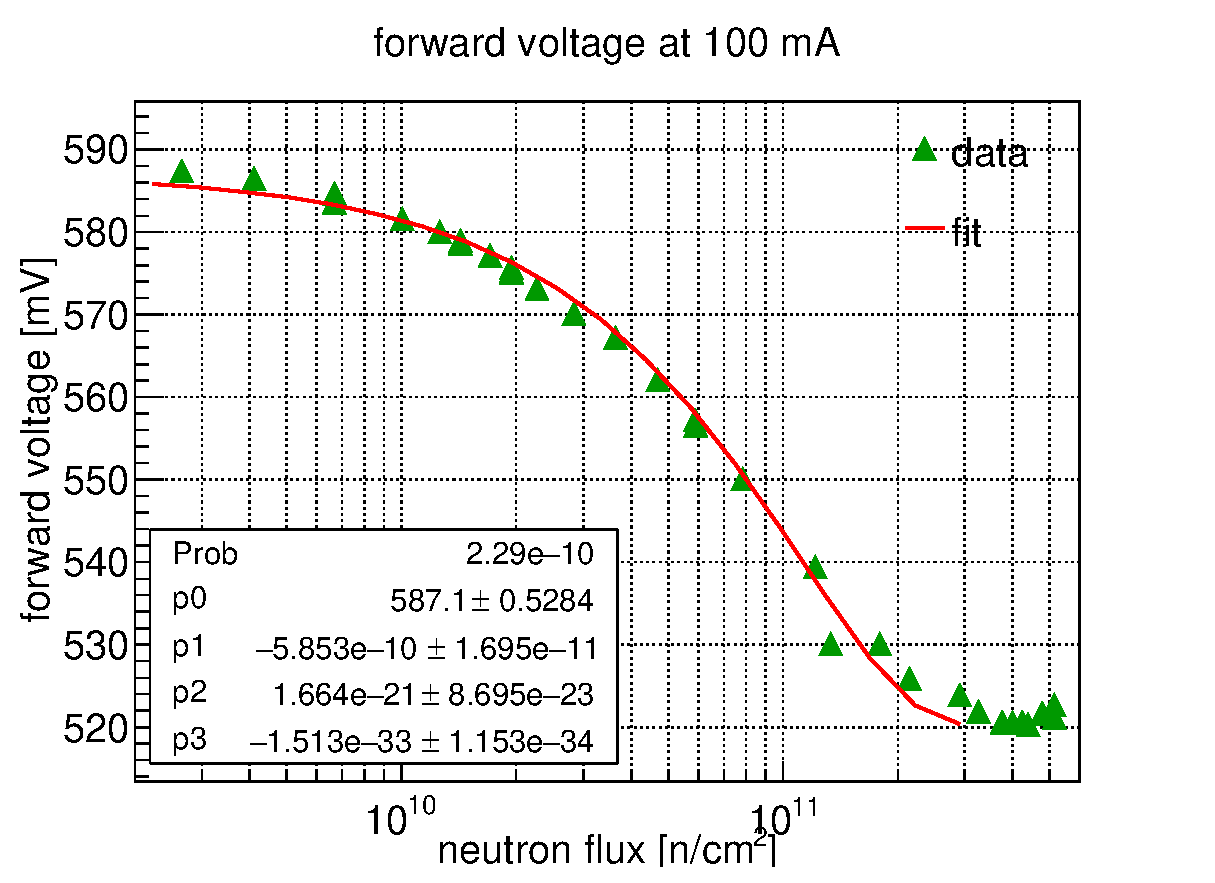
\includegraphics[scale=0.43]{chapter4/fig/switchon.eps}
   \end{subfigure}
   \caption{The temperature during the irradiation (left). The turn-on voltage decreases with the neutron fluence (right).}
   \label{3switch}
  \end{figure}
\begin{table}[H]
 \centering
 \begin{tabular}{cccccc} \hline \hline
  irradiated time [sec] & I$_0$ & V$_T$ & irradiated time [sec] & I$_0$ & V$_T$ \\ \hline
  0 & 2.04883$\times$10$^{-7}$ & 23.0918 & 500 & 1.97681$\times$10$^{-7}$ & 23.034 \\
  1064 & 2.73547$\times$10$^{-7}$ & 22.6213 & 1505 & 3.75863$\times$10$^{-7}$ & 22.2084 \\
  4274 & 1.35549$\times$10$^{-6}$ & 20.5447 & 9884 & 5.35415$\times$10$^{-6}$ & 18.7640 \\
  14008 & 9.77339$\times$10$^{-6}$ & 17.9582 & 68468 & 4.15128$\times$10$^{-5}$ & 15.7070 \\ \hline \hline
 \end{tabular}
 \caption{Fitting parameters for V-I curve.}
 \label{fit3}
\end{table}
  \begin{figure}[H]
   %\begin{subfigure}{0.3\textwidth}
    \centering
    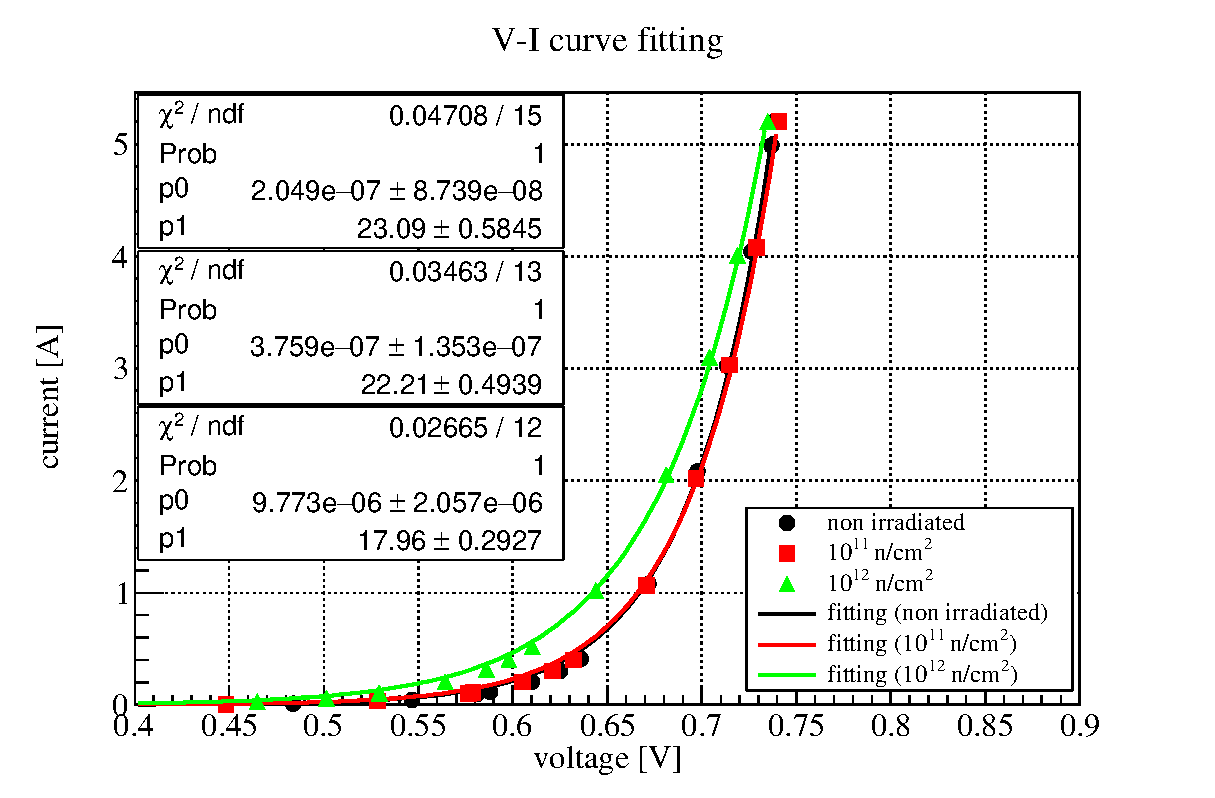
\includegraphics[scale=0.45]{chapter4/fig/diodefit.eps}
   %\end{subfigure}
   %\hspace{0.2\textwidth}
   %\begin{subfigure}{0.3\textwidth}
   % \centering
	%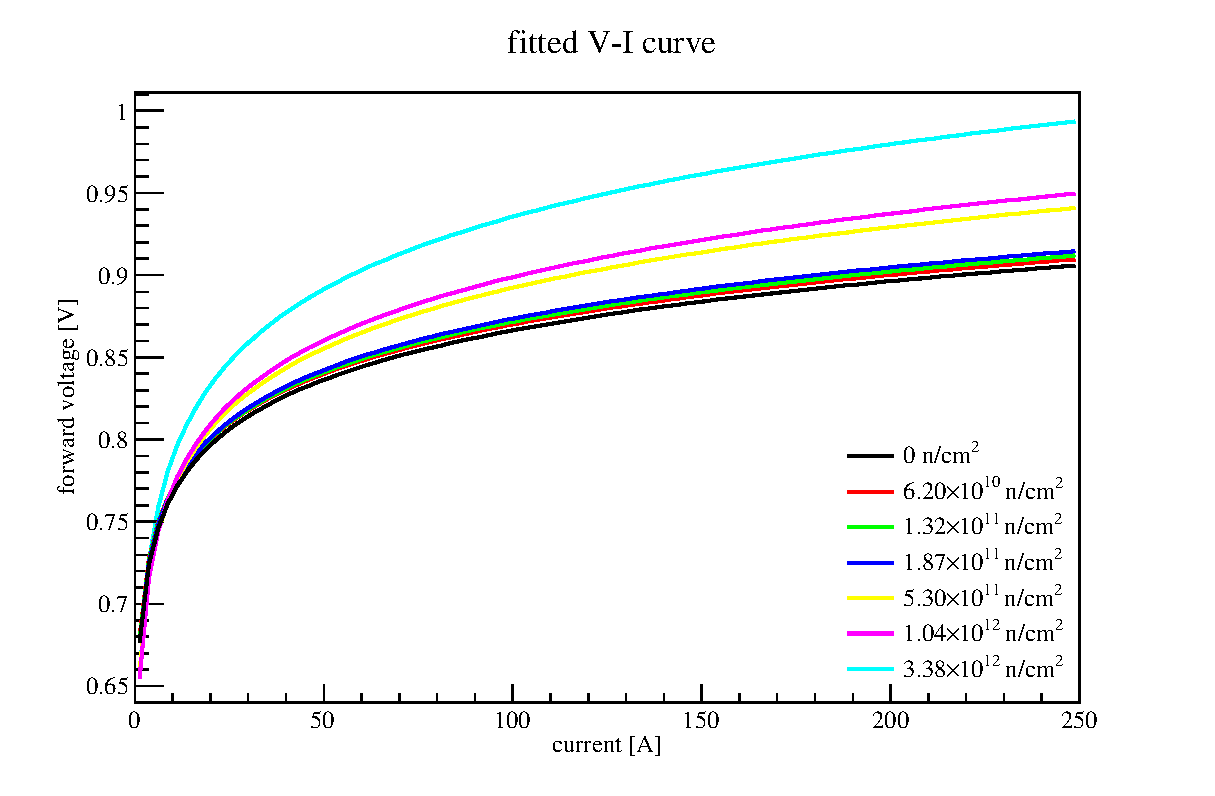
\includegraphics[scale=0.43]{chapter4/fig/fit210}
   %\end{subfigure}
   \caption{Measured turn-on voltage for quench protection diode. It is fitted as diode V-I function. Black and green point represent the original V-I curve and V-I curve after 10$^{12}$ n/m$^2$ irradiation.}
   \label{3fitdiode}
  \end{figure}
 
 \subsection{Electrical property at cryogenic temperature}
~~~~~Since Quench protection diode is connected to the magnets with superconducting wire, the diode must be cooled to the temperature same as superconducting wire, 4.2 K.
Therefore, the electrical property at cryogenic temperature needs to be investigated as well.

For the measurement at cryogenic temperature, Quench protection diode is cooled directly by liquid nitrogen at 77 K which shown in figure~\ref{3cryotemp}.
Unlike to the result of irradiation, not only the turn-on voltage but also the V-I curve increases in 77 K.
In figure~\ref{3cryo}, the V-I curve at 300 K and 7 K can be fitted by
\begin{table}[H]
 \centering
 \begin{tabular}{cccccc} \hline \hline
  Temperature [K] & I$_0$ & V$_T$ &Temperature [K] & I$_0$ & V$_T$ \\ \hline
  300 & 8.088$\times$10$^{-7}$ & 21.05 & 77 & 1.969$\times$10$^{-12}$ & 25.95 \\ \hline \hline
 \end{tabular}
 \caption{Fitting parameters for forward voltage of diode at 300 K and 77 K.}
 \label{fit4}
\end{table}
Using this fitting parameters, the forward voltage at 300 K and 77 K can be predicted to 0.92 V and 1.25 V respectively.
Compared with the case of room temperature, 0.33 V is increased during the cooling.
 \begin{figure}[H]
  \centering
  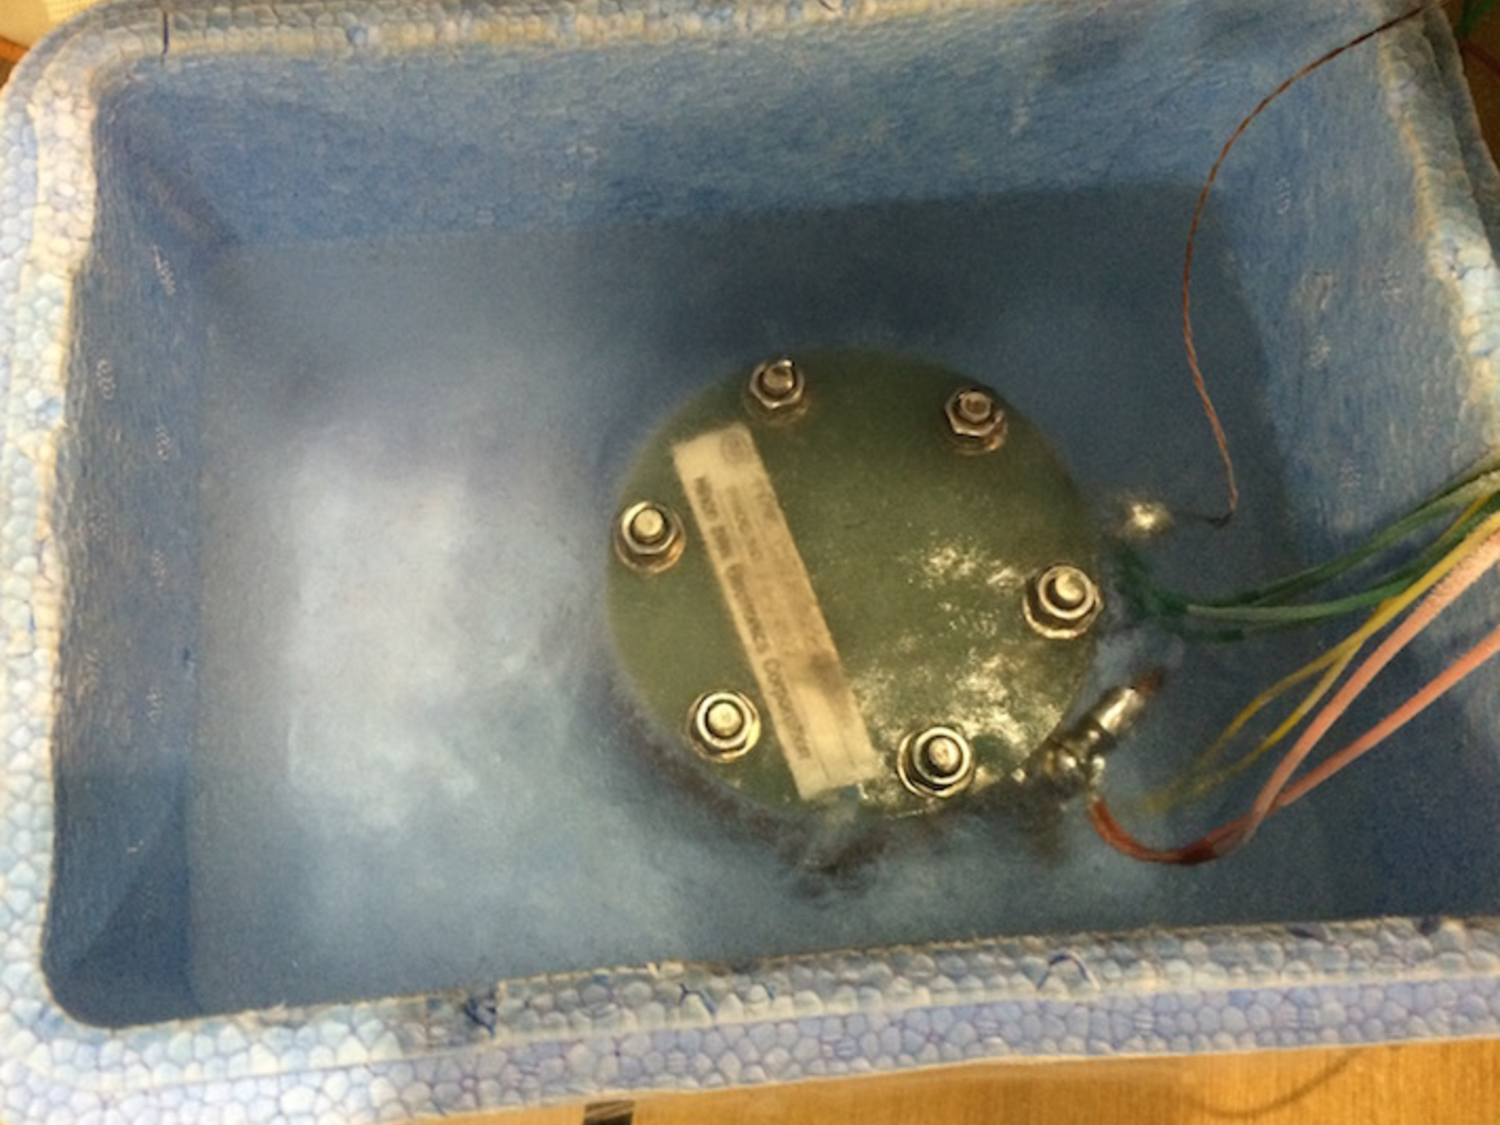
\includegraphics[scale=0.32]{chapter4/fig/cryotemp.pdf}
  \caption{Measurement of the forward voltage of diode at cryogenic temperature.}
  \label{3cryotemp}
 \end{figure}
 \begin{figure}[H]
  \begin{subfigure}{0.3\textwidth}
   \centering
   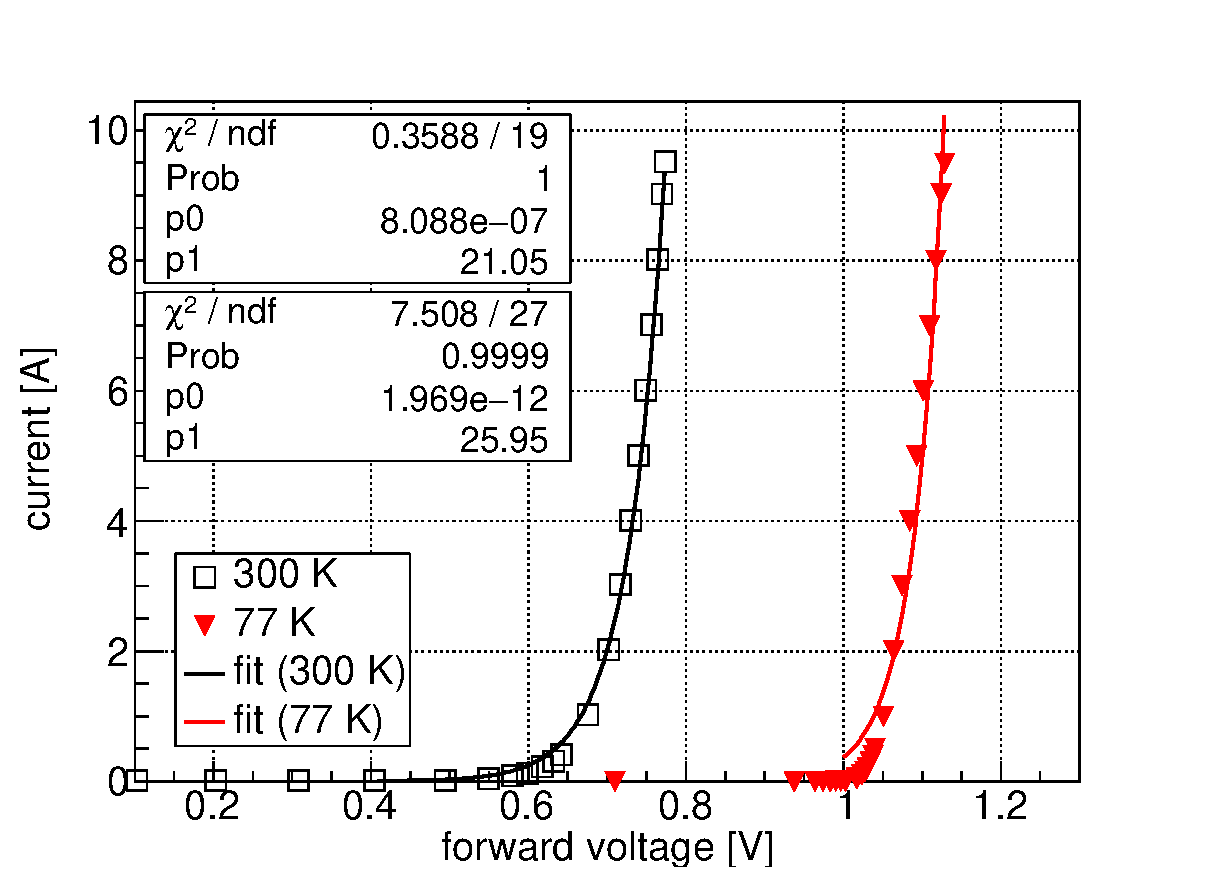
\includegraphics[scale=0.43]{chapter4/fig/cryo.eps}
  \end{subfigure}
  \hspace{0.2\textwidth}
  \begin{subfigure}{0.3\textwidth}
   \centering
   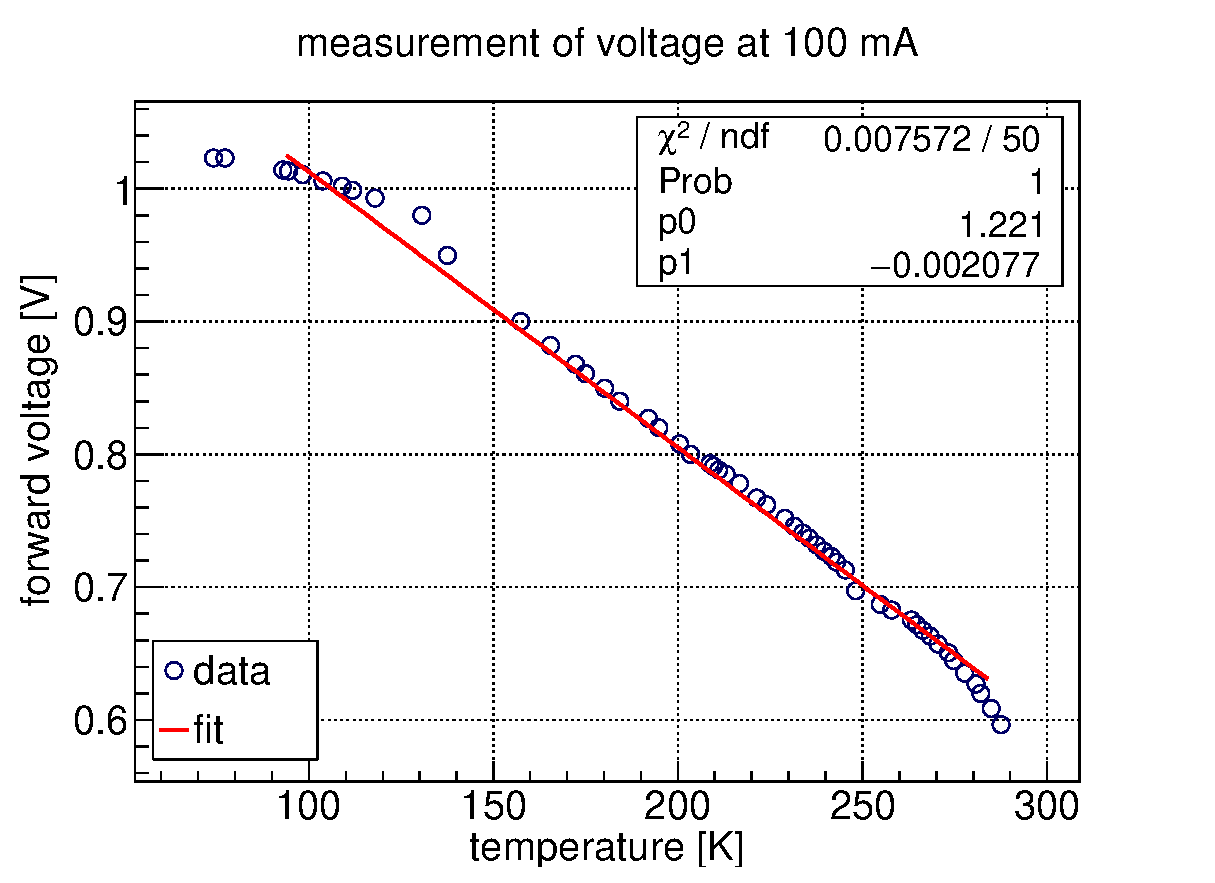
\includegraphics[scale=0.43]{chapter4/fig/temp.eps}
  \end{subfigure}
  \caption{Forward V-I curve measured at room temperature and nitrogen temperature without irradiation (left). The measurement of turn-on voltage at 100 mA from room temperature to 77 K (right).}
  \label{3cryo}
 \end{figure}

\subsection{Forward voltage at 210 A}
~~~~~~Since the operating current for transport solenoid is 210 A, a relation between fitted forward voltage at 210 A and neutron fluence is shown in figure~\ref{3diode}.
The forward voltage increases following the neutron fluence which is assumed as the exponential function.
\begin{equation}
 V = exp(-0.09373 + 8.832 \times 10^{-14} \cdot \phi)
\end{equation}
In the case of COMET phase-II experiment, the neutron at the place of quench protection diode is about 4.02$\times$10$^5$ n/cm$^2$/sec with the energy lower than 1 MeV  according to PHITS simulation.
As for the 280-day operation, the total neutron fluence is estimated to about 9.73$\times$10$^{12}$ n/cm$^2$ for quench protection diode.
Because the displacement cross section of silicon at low energy region is lower than the case of high energy region, irradiation for 10$^{12}$ n/cm$^2$ at the range from 1 MeV reaches to the effects of 9.73$\times$10$^{12}$ n/cm$^2$ irradiation.
After 10$^{12}$ n/cm$^2$ irradiation, the forward voltage at operating current is increased 0.08 V.
  \begin{figure}[H]
   \centering
   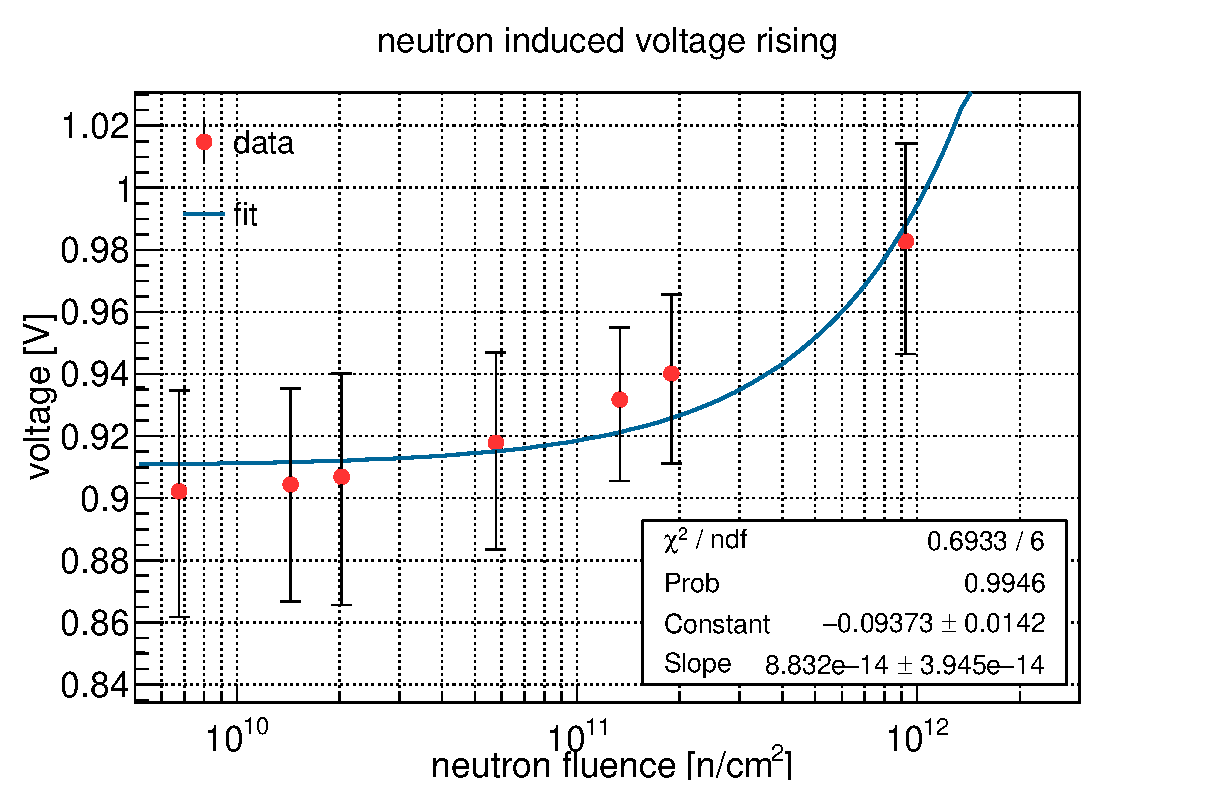
\includegraphics[scale=0.5]{chapter4/fig/dioderesult.eps}
   \caption{Relative increase of the forward voltage versus neutron fluence at room temperature.}
   \label{3diode}
  \end{figure}

Turn-on voltage at 100 mA is proportional to the temperature linearly as
\begin{equation}
 V = 1.221 - 0.002077 \cdot T
\end{equation}
Assuming the forward voltage at 210 A is also linear to the temperature, the forward voltage is predicted to 1.33 V at 4.2 K and 210 A without irradiation.

However, the forward voltage is estimated to 0.98 V at 210 A and room temperature after irradiation of 10$^{12}$ n/cm$^2$ neutrons.
Supposed its forward voltage is 1.5 V at 4.2 K and 210 A with irradiation of 10$^{12}$ n/cm$^2$ neutrons, its heat generation is the product of forward voltage and current, which is 315 W.
The temperature of quench protection diode is calculated by one dimensional finite element method.
Diode consists of silicon with length of 8 cm and radius of 3 cm.
Its thermal conductivity shown in figure~\ref{sicond} is taken and fitted from reference~\cite{glass}\cite{holl}.
Two sides of diode is cooled by liquid helium at 4.2 K, and heat is generated inside the diode.
Current decays with the resistance of heater ($R$ = 2.38 $\Omega$, $L$ = 254 $H$).
As a result, the maximum temperature will be 11 K during the cooling.
Without the cooling, the temperature of diode will increase up to 70 K at 10 sec.
\begin{figure}[H]
  \centering
  \includegraphics[scale=0.42]{chapter4/fig/thermalcond.eps}
  \caption{Experimental data of the thermal conductivity for silicon.}
  \label{sicond}
\end{figure}
To confirm the temperature, the temperature of quench protection diode is also estimated by ANSYS.
The thermal conductivity is approached linearly between the two data points.
Diode is cooled by liquid helium at 4.2 K on the top and bottom of surface.
Heat generation is set to 315 W homogeneously without current decay, which is the worst circumstance for diode.
As a result, it maximum temeprature is about 6.0 K.
\begin{figure}[H]
 \centering
 \includegraphics[scale=0.38]{chapter4/fig/diode000.pdf}
 \caption{The temperature distribution of quench protection diode during the operation calculated by ANSYS.}
 \label{ansys}
\end{figure}
%Including the voltage change during the irradiation, we assume the forward voltage at 210 A and 4.2 K will increase from 0.9 V to 1.5 V.
%Even if the forward voltage increases to 1.5V, the temperature rises to about 11 K during the cooling of liquid helium which is calculated by one dimensional Finite Element Method.
%Without the cooling, the temperature of diode will increase up to 70 K at 10 sec.


 \section{Radiation test for conductor}
~~~~~~The degradation of electrical resistivity occurs when the stabilizer irradiated by radiation due to the production of Frenkel pairs.
In the cryogenic temperature, since the displaced atoms are difficult to return to the defect, a depletion region is possible to be generated under the long time irradiation.
Radiation damage effects of conductor are necessary to investigate because it may cause the overheat of superconducting coils due to the RRR decreasing and quench.
\begin{figure}[H]
 \begin{subfigure}{0.3\textwidth}
  \centering
  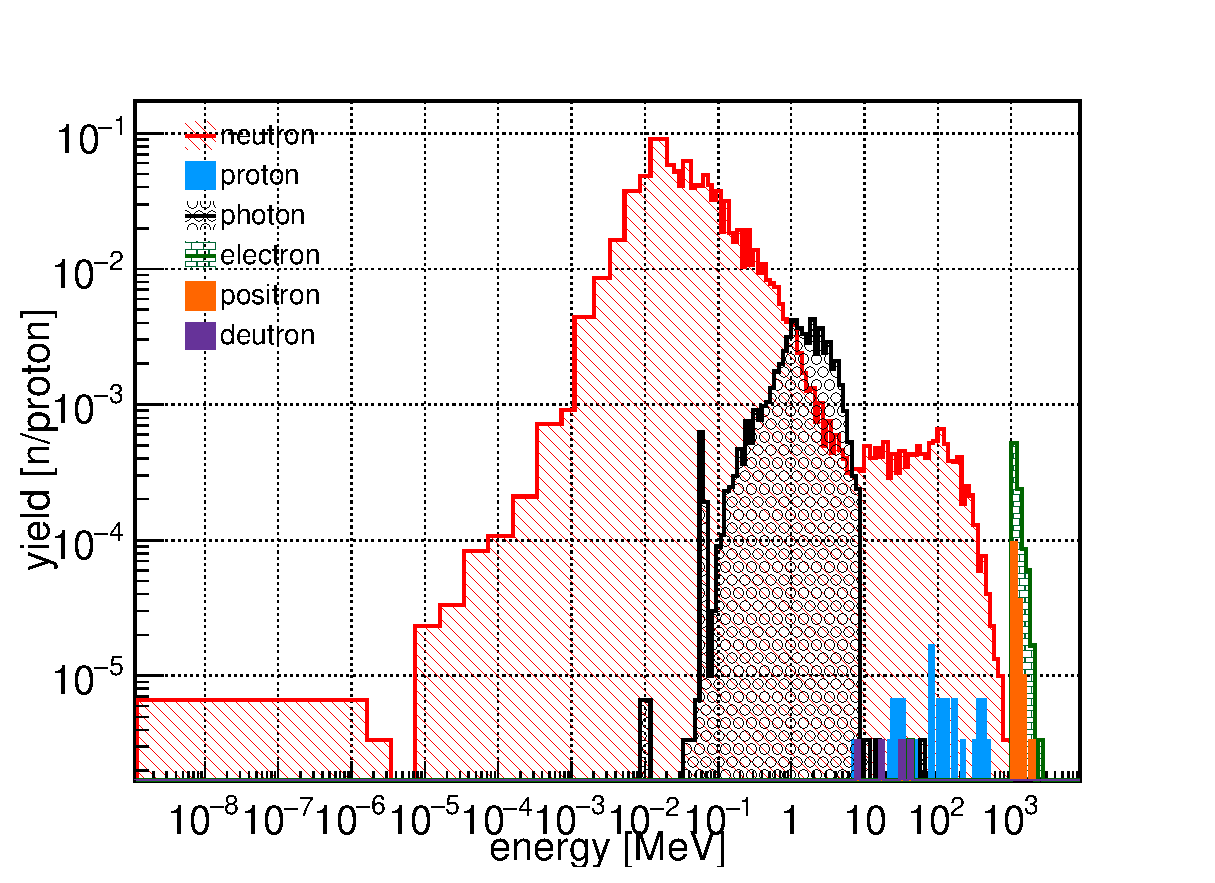
\includegraphics[scale=0.43]{chapter4/fig/yield.eps}
 \end{subfigure}
 \hspace{0.2\textwidth}
 \begin{subfigure}{0.3\textwidth}
  \centering
  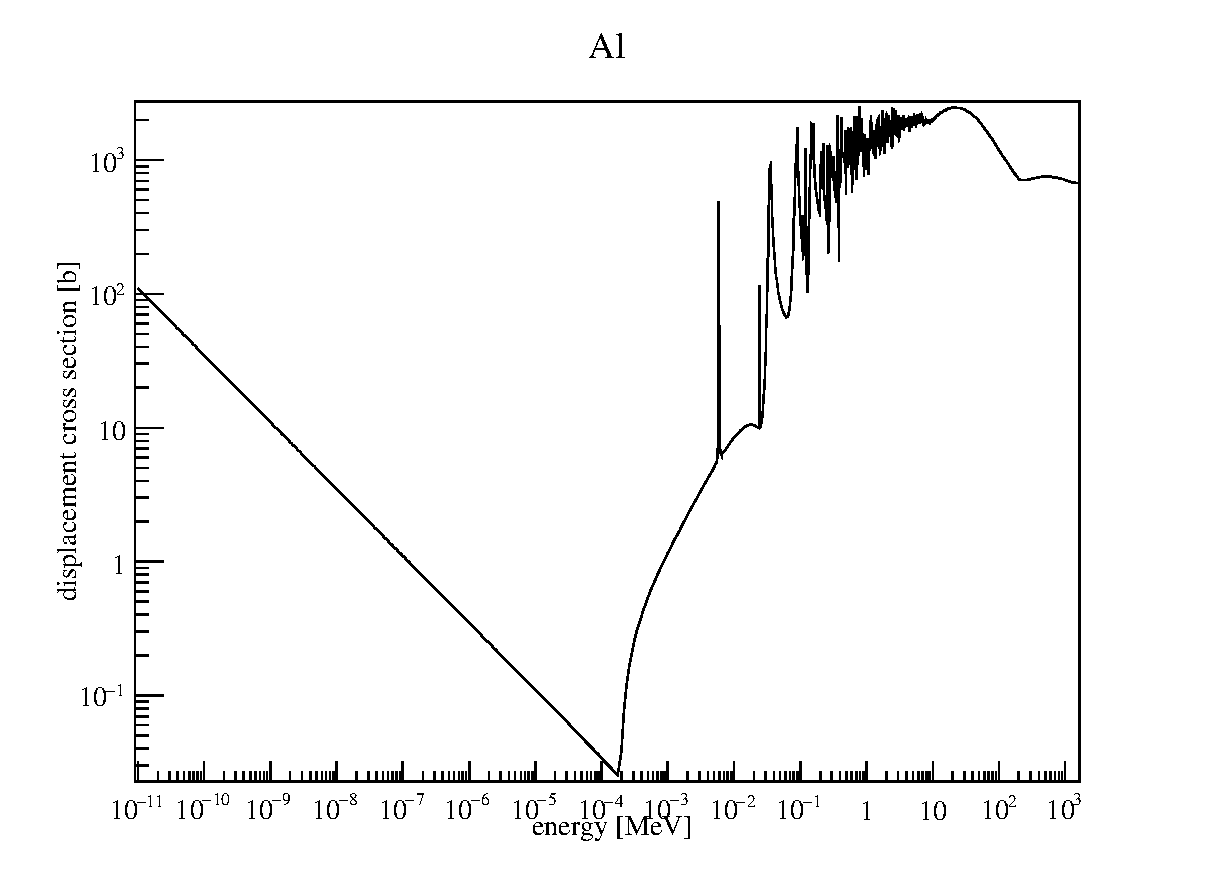
\includegraphics[scale=0.43]{chapter5/fig/AlDPA.eps}
 \end{subfigure}
 \caption{all kinds of particles which hit the CS1 coil (left). The displacement cross section of aluminium for neutron (right).}
 \label{3yield}
\end{figure}
  \begin{figure}[H]
    \centering
	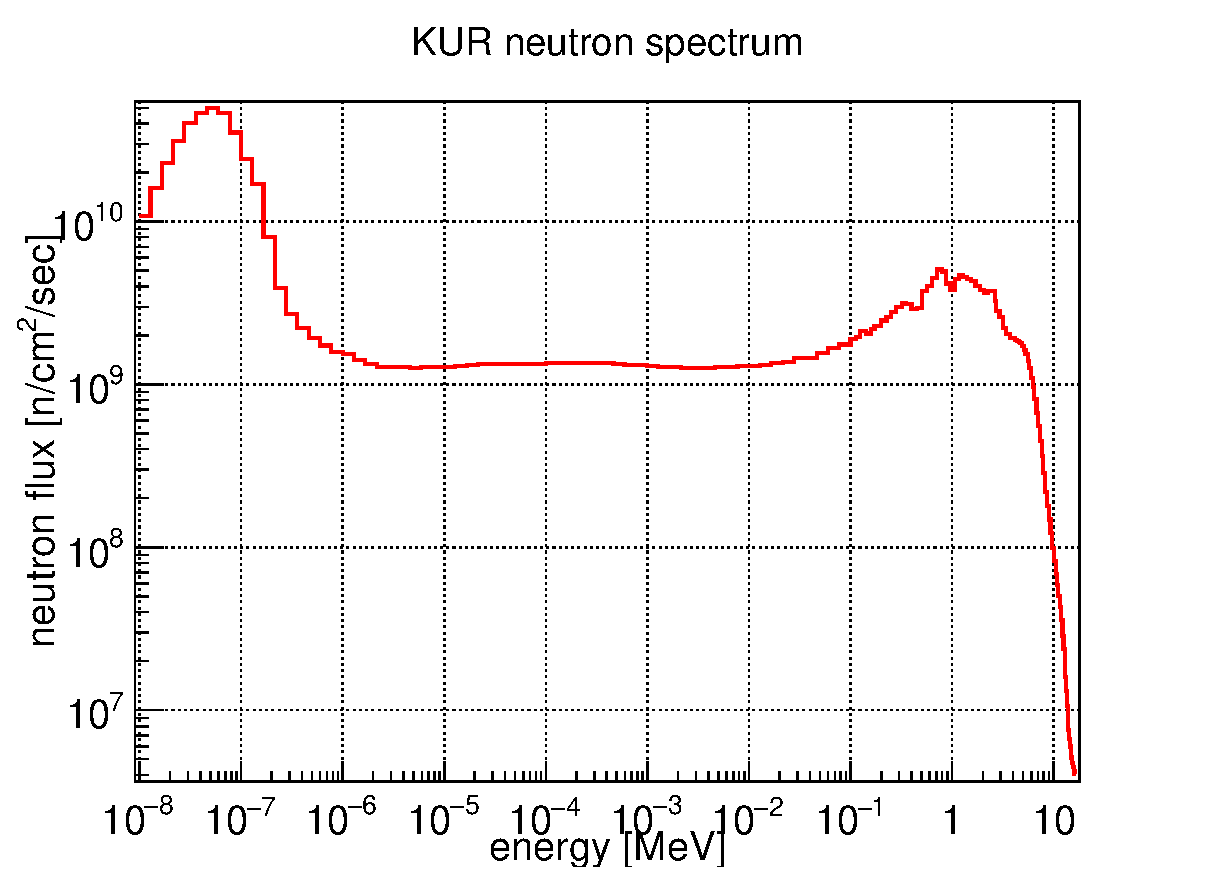
\includegraphics[scale=0.43]{chapter5/fig/neutron.eps}
   \caption{Neutron spectrum at core of KUR reactor.}
   \label{4dpa}
  \end{figure}
To ensure what kinds of particle hit the superconducting coils, the simulation is taken by PHITS and its yield is shown in figure~\ref{3yield}.
Compared with the other particles, the neutron is most biggest issue for superconducting coils.
Furthermore, the energy of neutron in the range from 0.1 MeV dominates the radiation damage, which is about 100 b.
Thus, irradiation test of pure aluminium and copper for conductor is studied in Kyoto University Research Reactor Institute (KURRI) with reactor neutron.
The pure aluminium and copper samples are set up in the one of beamline from reactor where can irradiate with cryogenic temperature.
Neutron fluence is 1.4$\times$10$^{11}$ n/m$^2$/sec for fast neutron in terms of the KUR study~\cite{kur}.
Figure~\ref{4dpa} shows the energy spectrum at center of reactor, which is higher than the place where we take irradiation test with factor 30.34.

As the result, we obverse that the resistivity increases about 0.03 n$\Omega\cdot$m for aluminium and 0.01 n$\Omega\cdot$m for copper after after 10$^{20}$ n/m$^2$ neutron irradiation.
Thus, due to the neutron induced resistivity, the resistivity of stabilizer at cryogenic temperature should be modified as
\begin{equation}
 \rho (T) = \rho_0(T) + \Delta \rho_{n} (\Phi) + \Delta \rho_{mag} (B)
\end{equation}
where $\rho_0(T)$ is the resistivity at cryogenic temperature without magnetic field and irradiation.
$\Delta \rho(\Phi)$ and $\Delta \rho(B)$ are the neutron induced resistivity which depends on the neutron fluence and magnetoresistivity, respectively.
Thus, the RRR during the irradiation is given by
\begin{equation}
 RRR = \frac{\rho_{RT}}{\rho_0 + f \cdot \phi \cdot t}
\end{equation}
where the factor $f$ is shown in table~\ref{factorirr}.
\begin{table}[H]
 \centering
 \begin{tabular}{cc} \hline \hline
  Element & Factor [n$\Omega\cdot$m$^3$] \\ \hline
  aluminium & 3$\times$10$^{-22}$ \\
  Copper & 1$\times$10$^{-22}$ \\ \hline \hline
 \end{tabular}
 \caption{Factor for the neutron induced resistivity.}
 \label{factorirr}
\end{table}
Since the aluminium with RRR of 2000 and 400 will be employed as strip and stabilizer respectively, the relation between RRR and neutron fluence is shown in figure~\ref{4rrr}.
The RRR of aluminium strip and stabilizer for 280-day operation will become 40 or lower for capture solenoid according to the maximum neutron fluence of 2$\times$10$^{21}$ n/m$^2$ which is predicted by PHITS code (JAM\_INCL4.6\_JENDL4 model).
Details of RRR degradation for main superconducting magnets of pion capture solenoid is listed in table~\ref{RRRdeg} and figure~\ref{4rrr} (right).
 \begin{figure}[H]
   \begin{subfigure}{0.3\textwidth}
    \centering
	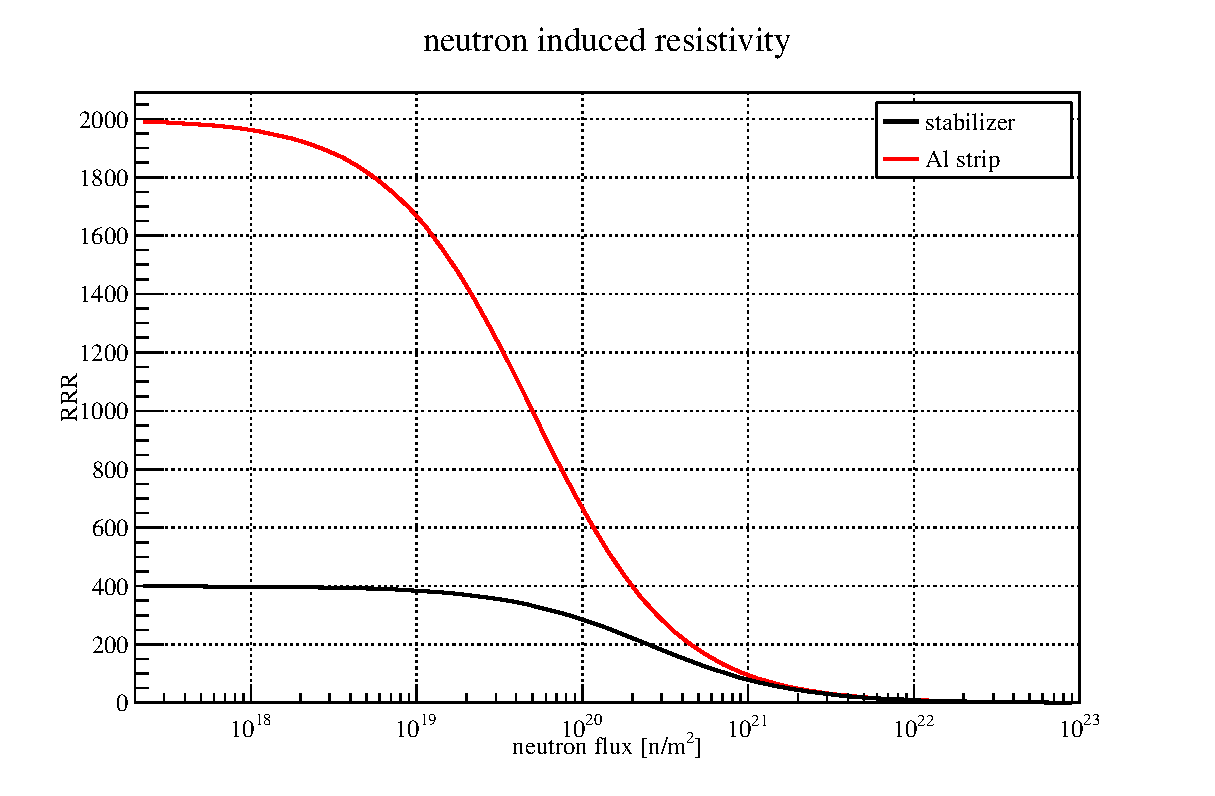
\includegraphics[scale=0.43]{chapter5/fig/degradation.eps}
   \end{subfigure}
   \hspace{0.2\textwidth}
   \begin{subfigure}{0.3\textwidth}
    \centering
	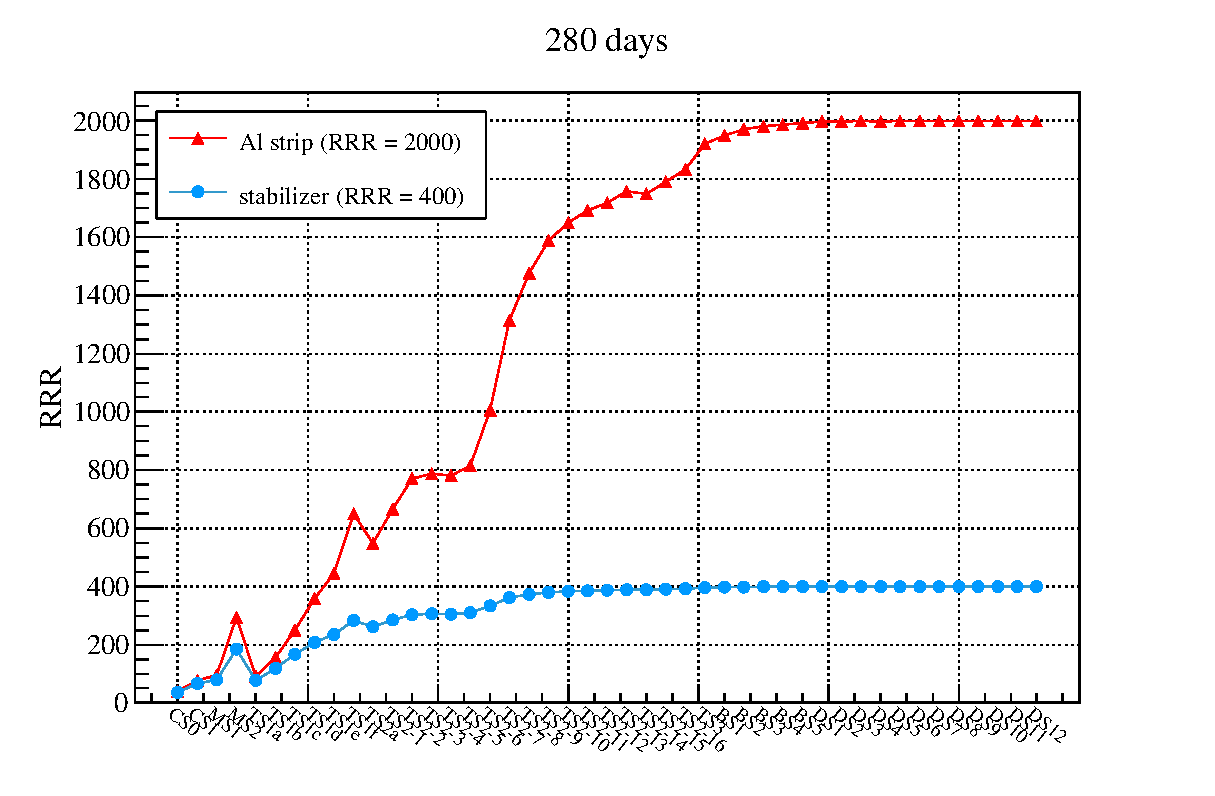
\includegraphics[scale=0.43]{chapter5/fig/rrrmagnets.eps}
   \end{subfigure}
   \caption{ Predicted the RRR-neutron curve from the neutron irradiation test in KUR.}
   \label{4rrr}
  \end{figure}

\begin{table}[H]
 \centering
 \begin{tabular}{ccccc} \hline \hline
  Name & neutron flux [n/cm$^2$/sec] & DPA [DPA/280 days] & RRR (Al strip) & RRR (stabilizer) \\ \hline
  CS0 & 1.03$\times$10$^{10}$ & 3.44$\times$10$^{-5}$ & 39 & 36 \\
  CS1 & 5.12$\times$10$^{9}$ & 2.97$\times$10$^{-5}$ & 77 & 67 \\
  MS1 & 4.11$\times$10$^{9}$ & 1.82$\times$10$^{-5}$ & 95 & 80 \\
  MS2 & 1.20$\times$10$^{9}$ & 8.11$\times$10$^{-6}$ & 293 & 185 \\ \hline \hline
 \end{tabular}
 \caption{Details of RRR degradation for pion capture solenoid after 280-day operation.}
 \label{RRRdeg}
\end{table}

 \subsection{Discussion}
~~~~~~The radiation induced damage of material can be estimated by one parameter called Displacement Per Atom (DPA) which is given by
\begin{equation}
 DPA = \sigma_{dpa} \cdot \phi_i
\end{equation}
where $\sigma_{dpa}$ and $\phi_i$ are the displacement cross section and particle flux respectively.
The displacement cross section depends on the material, and is a predicting value.
Through the DPA, the radiation damage in different energy region is able to be compared.
Using the neutron flux and displacement cross section of aluminium in figure~\ref{3yield} and the neutron spectrum of KUR, the DPA for KUR irradiation test can be estimated as follows.
\begin{table}[H]
 \centering
 \begin{tabular}{cc} \hline \hline
  DPA model & DPA calculation [DPA] \\ \hline
  BCA + MD & 1.0$\times$10$^{-5}$ \\
  ABBN & 2.6$\times$10$^{-5}$ \\
  NRT (Mu2e) & 2.5$\times$10$^{-5}$ \\
  NRT (COMET) & 3.0$\times$10$^{-5}$ \\ \hline \hline
 \end{tabular}
 \caption{DPA estimation for the neutron irradiation test of pure aluminium. NRT (COMET) is estimated PHITS code, and the others are predicted by Mu2e collaboration with same experiment.}
\end{table}
\begin{table}[H]
 \centering
 \begin{tabular}{ccc} \hline \hline
  $\rho_{FP}$ [$\mu\Omega\cdot$m] & Type & Reference \\ \hline
  3.9$\pm$0.6 & Exp D & \cite{erh1} \\
  4.2$\pm$0.8 & Exp D & \cite{erh2} \\
  3.2$\pm$0.6 & Exp D & \cite{rober} \\
  3.4 & Exp T(p) & \cite{ref1} \\
  1.32 & Exp T(p) & \cite{ref2} \\
  1.35 & Exp T(p) & \cite{ref3} \\
  4.0$\pm$0.6 & Evl E & \cite{ref4} \\
  4.2$\pm$0.5 & Evl E & \cite{ref5} \\
  4.3 & Evl S & \cite{ref6} \\ 
  6.8 & Adp & \cite{horak} \\
  2.0$\pm$1.0 & KEK & \\ \hline \hline
 \end{tabular}
 \caption{The Frenkel pair resistivity $\rho_{FP}$ of aluminium. Methods of the data derivation: Exp D is X-ray diffraction method, Exp T is the threshold energy determination for electron irradiation of single crystals at low temperature. Exp T(p) is for the electron irradiation of polycrystals, Evl S is the estimation made with the help of the systematics. Adp is the data adopted by the authors of cited work~\cite{yu}. KEK is the neutron irradiation test in KUR.}
 \label{frank}
\end{table}
Here, BCA + MD, ABBN, and NRT (Mu2e) are the estimation with different DPA models from Mu2e collaboration.
Our estimation is about 3.0$\times$10$^{-5}$ DPA.
J.A. Horak et al. measure the neutron induced resistivity of metals, as a result, the induced resistivity for aluminium is 382.3 n$\Omega\cdot$cm per 5.6$\times$10$^{-4}$ Frenkel pair~\cite{horak}.
In addition, reference~\cite{yu} shows many results of Frenkel pair resistivity of aluminium in table~\ref{frank}.
It shows that J.A. Horak's data is the maximum value compared with the other references.
The relation between DPA and RRR by using these prediction from experimental data is shown in~\ref{dpaaa}.

For the COMET phase-II experiment, the DPA peak of CS1 coil is about 1.1$\times$10$^{-5}$ DPA for 280-day operation from the prediction of PHITS code with NRT model.
The aluminium strip will not degrade lower than 100 for 280-day operation from this estimation.
However, the design has to consider the worst situation for superconducting coils, the uncertainty of the prediction from neutron DPA and neutron fluence needs to be reconsidered.
\begin{figure}[H]
 \centering
 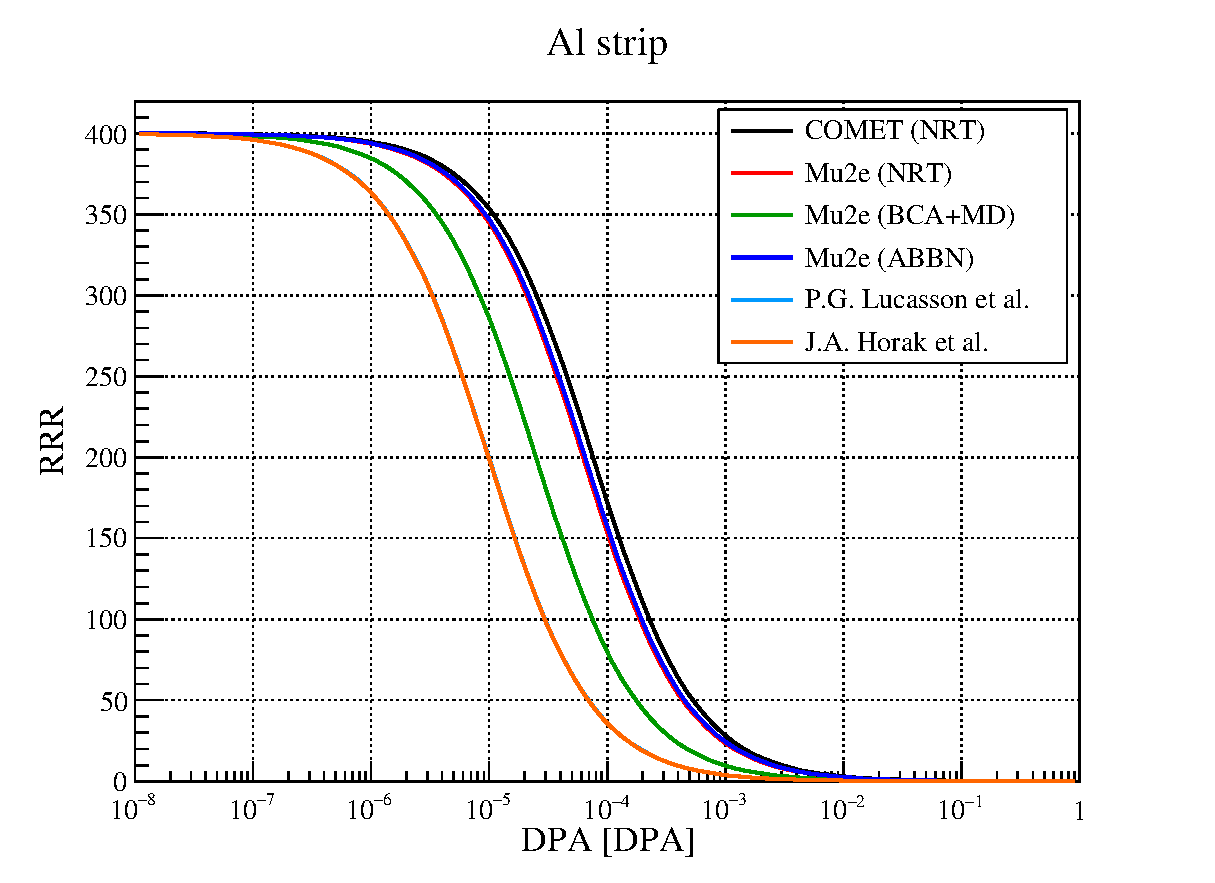
\includegraphics[scale=0.5]{chapter4/fig/dpadegradation.eps}
 \caption{A relation between DPA and RRR. Orange line is the maximum radiation induced resistivity, and the others are the prediction of KUR irradiation test with different displacement cross section model.}
 \label{dpaaa}
\end{figure}
